% The packages used here are just a sample. You may need others, and may not need some of these. It doesn't hurt to leave them in, unless they start to conflict with other packages you've added. Chapter 2 has example code for equations, figures, tables, citations, abbreviations, etc. If there are sections labeled 'optional' that you don't want, just comment them out. -jg

\documentclass[reqno,12pt,oneside]{report} % right-side equation numbering, 12 point font, print one-sided 
%\documentclass[reqno,12pt,twoside,openright]{report} % right-side equation numbering, 12 point font, print two-sided, Chapters start on odd pages. Rackham only accepts one-sided, so this is for personal printings.

\usepackage{rac}         % Use Rackham thesis style file
\usepackage{aas_macros}  % To allow the reading of ADS journal references in the bibliography
%\usepackage[intlimits]{amsmath} % Puts the limits of integrals on top and bottom
\usepackage{amsxtra}     % Use various AMS packages
\usepackage{amsthm}
\usepackage{amssymb}
\usepackage{amsfonts}
\usepackage{graphicx}    % Add some packages for figures. Read epslatex.pdf on ctan.tug.org
\usepackage{rotating}
\usepackage{color}
\usepackage{epsfig}
\usepackage{subfigure}   % To make subfigures. Read subfigure.pdf on ctan.tug.org
%\usepackage{caption}
%\usepackage{subcaption}
\usepackage{verbatim}
\usepackage{natbib}      % Allows you to use BibTeX
\usepackage[printonlyused]{acronym} % For the List of Abbreviations. Read acronym.pdf on ctan.tug.org
\usepackage{setspace}    % Allows you to specify the line spacing
\newcommand{\fixme}[1]{\textbf{\textcolor{red}{[Fixme: #1]}}}
\newcommand{\NVDisk}{{\em NVRAM Disk-Rep\-lace\-ment}\xspace}
\newcommand{\InPlace}{{\em In-Pl\-ace Up\-dat\-es}\xspace}
\newcommand{\GroupCommit}{{\em NVRAM Group Com\-mit}\xspace}

\usepackage{textcomp}
\usepackage{txfonts}
\usepackage{booktabs}
\usepackage{multirow}

%\doublespacing           % \onehalfspacing for 1.5 spacing, \doublespacing for 2.0 spacing.
\onehalfspacing
%\newcommand{\sun}{\ensuremath{\odot}} % sun symbol is \sun
%%%%%%%%%%%%%%%%%%%%%%%%%%%%%%%%%%%%%%%%%%%%%%%%%%%%%%%%%%%%%%%%%%%%%%%%%%%%%%%

% Various theorem environments. All of the following have the same numbering
% system as theorem.

\theoremstyle{plain}
\newtheorem{theorem}{Theorem}
\newtheorem{prop}[theorem]{Proposition}
\newtheorem{corollary}[theorem]{Corollary}
\newtheorem{lemma}[theorem]{Lemma}
\newtheorem{question}[theorem]{Question}
\newtheorem{conjecture}[theorem]{Conjecture}
\newtheorem{assumption}[theorem]{Assumption}

\theoremstyle{definition}
\newtheorem{definition}[theorem]{Definition}
\newtheorem{notation}[theorem]{Notation}
\newtheorem{condition}[theorem]{Condition}
\newtheorem{example}[theorem]{Example}
\newtheorem{introduction}[theorem]{Introduction}

\theoremstyle{remark}
\newtheorem{remark}[theorem]{Remark}
%%%%%%%%%%%%%%%%%%%%%%%%%%%%%%%%%%%%%%%%%%%%%%%%%%%%%%%%%%%%%%%%%%%%%%%%%%%%%%%

\numberwithin{theorem}{chapter}     % Numbers theorems "x.y" where x
                                    % is the section number, y is the
                                    % theorem number

%\renewcommand{\thetheorem}{\arabic{chapter}.\arabic{theorem}}

%\makeatletter                      % This sequence of commands will
%\let\c@equation\c@theorem          % incorporate equation numbering
%\makeatother                       % into the theorem numbering scheme

%\renewcommand{\theenumi}{(\roman{enumi})}

%%%%%%%%%%%%%%%%%%%%%%%%%%%%%%%%%%%%%%%%%%%%%%%%%%%%%%%%%%%%%%%%%%%%%%%%%%%%%%

% If printing two-sided, this makes sure that any blank page at the 
% end of a chapter will not have a page number. 
\makeatletter
\def\cleardoublepage{\clearpage\if@twoside \ifodd\c@page\else
\hbox{}
\thispagestyle{empty}
\newpage
\if@twocolumn\hbox{}\newpage\fi\fi\fi}
\makeatother 

%%%%%%%%%%%%%%%%%%%%%%%%%%%%%%%%%%%%%%%%%%%%%%%%%%%%%%%%%%%%%%%%%%%%%%%%%%%%%%

%This command creates a box marked ``To Do'' around text.
%To use type \todo{  insert text here  }.

\newcommand{\todo}[1]{\vspace{5 mm}\par \noindent
\marginpar{\textsc{To Do}}
\framebox{\begin{minipage}[c]{0.95 \textwidth}
\tt\begin{center} #1 \end{center}\end{minipage}}\vspace{5 mm}\par}

%%%%%%%%%%%%%%%%%%%%%%%%%%%%%%%%%%%%%%%%%%%%%%%%%%%%%%%%%%%%%%%%%%%%%%%%%%%%%%%
\begin{document}

\bibliographystyle{agu04}    % Set the bibliography style. agu04, plain, alpha, etc.

% Title page as required by Rackham dissertation guidelines
\titlepage{Thesis Proposal: Database and System Design for Emerging Storage Technologies}{Steven Pelley}{Doctor of Philosophy}
{Computer Science and Engineering}{2013}
{Assistant Professor Thomas F. Wenisch, Chair\\
 Professor Peter M. Chen\\
 Assistant Professor Michael J. Cafarella\\
 Assistant Professor Zhengya Zhang}

% Begin the front matter as required by Rackham dissertation guidelines
\initializefrontsections

% Optional Frontispiece
%\frontispiece{
\includegraphics[width=6in]{Intro/Happy} Find a cool picture to go here.}

% Optional, but recommended, Copyright page
%\copyrightpage{Steven Pelley}

% Page numbering. If you don't include a frontispiece or copyright page, you'll need to change this for two-sided printing.
\makeatletter
\if@twoside \setcounter{page}{4} \else \setcounter{page}{0} \fi
\makeatother
 
% Optional Dedication page
%\dedicationpage{For all the people}

% Optional Acknowledgements page
%\startacknowledgementspage
%Thanks to the people who made this dissertation possible, especially those who put together a nice \LaTeX\, template for me to use.
%\label{Acknowledgements}

% Optional Preface page
%\startprefacepage
%\input{Preface}
%\label{Preface}

% Table of contents, list of figures, etc.
\tableofcontents     % Required
\listoffigures       % Required if there is more than one figure
\listoftables        % Required if there is more than one table
%\listofmaps          % Required if there is more than one map
\listofappendices    % Required if there is more than one appendix
\listofabbreviations % Optional. Abbreviations should be stored in a file named abbr.tex

% Optional in-dissertation Abstract Page
\startabstractpage
{Database and System Design for Emerging Storage Technologies}{Steven Pelley}{Chair: Thomas F. Wenisch}
Emerging storage technologies offer an alternative to disk that is durable and allows faster data access.
Flash memory, made popular by mobile devices, provides block access with low latency random reads.
New nonvolatile memories (NVRAM) are expected in upcoming years, presenting DRAM-like performance alongside persistent storage.
Wheres both technologies accelerate data accesses due to increased raw speed, used merely as disk replacements they may fail to achieve their full potentials.
Flash's asymmetric read/write access (i.e., reads execute faster than writes) opens new opportunities to optimize Flash-specific access.
Similarly, NVRAM's low latency persistent accesses allow new designs for high performance failure-resistant applications.

This thesis addresses software and hardware system design for such storage technologies.
First, I investigate analytics query optimization for Flash, expecting Flash's fast random access to require new query planning.
While intuition suggests scan and join selection should shift between disk and Flash, I find that query plans chosen assuming disk are already near-optimal for Flash.
Second, I examine new opportunities for durable, recoverable transaction processing with NVRAM.
Existing disk-based recovery mechanisms impose large software overheads, yet updating data in-place requires frequent device synchronization that limits throughput.
I introduce a new design, \GroupCommit, to amortize synchronization delays over many transactions, increasing throughput at some cost to transaction latency.
Finally, I propose a new framework for persistent programming and memory systems to enable high performance recoverable data structures with NVRAM, extending memory consistency with persistent semantics to introduce \emph{memory persistency}.

\label{Abstract}

\startthechapters 
% The individual files for each of the chapters are put here.
% Save each chapter of your thesis to a seperate tex file
% and then use the \input command to include this file in your
% thesis.  For instance you can save a file to "intro.tex" and 
% then type \section{Introduction}

Data center power consumption continues to grow at an alarming pace; it is projected to reach 100 billion kWh at an annual cost of \$7.4 billion within two years \cite{EPA07}, with a world-wide carbon-emissions impact similar to that of the entire Czech Republic \cite{Mankoff08}. In light of this trend, computer systems researchers, application designers, power and cooling engineers, and governmental bodies have all launched research efforts to improve data center energy efficiency.  These myriad efforts span numerous aspects of data center design (server architecture \cite{Lefurgy03,Meisner09}, scheduling \cite{Moore06, Parolini08},  power delivery systems \cite{Fan07}, cooling infrastructure \cite{Patel02}, etc.).  However, with few exceptions, existing efforts focus narrowly on energy-efficiency of single subsystems, without considering global interactions or implications across data center subsystems. 

As sophisticated power management features proliferate, the dynamic range of data center power draw (as a function of utilization) is increasing, and interactions among power management strategies across subsystems grow more complex; subsystems can no longer be analyzed in isolation.   Even questions that appear simple on their face can become quite complicated.

Reasoning about total data center power is difficult because of the diversity and complexity of data center infrastructure.  Five distinct sub-systems (designed and marketed by different industry segments) account for most of a data center's power draw:  (1) servers and storage systems, (2) power conditioning equipment, (3) cooling and humidification systems, (4) networking equipment, and (5) lighting/physical security.  Numerous sources have reported power breakdowns \cite{EPA07,Meisner09}; Table~\ref{table::PowerDistribution} illustrates a typical breakdown today.   The first three subsystems dominate and their power draw can vary drastically with data center utilization. Cooling power further depends on ambient weather conditions around the data center facility. Even the distribution of load in each subsystem can affect power draws, as the interactions among sub-systems are non-linear
%(e.g., thermal hot spots disproportionately increase cooling requirements).

In this paper, our objective is to provide tools to the computer systems community to assess and reason about total data center power.  Our approach is two-fold, targeting both \emph{data center simulation} and \emph{abstract analytic modeling}.  First, we have collected a set of detailed power models (from academic sources, industrial white papers, and product data sheets) for each critical component of data center infrastructure, which describe power draw as a function of environmental and load parameters.  Each model describes the power characteristics of a single device (i.e., one server or computer room air handler (CRAH)) and, as such, is suitable for integration into a detailed data center simulator.  We describe how these models interact (i.e., how utilization, power, and heat flow among components) and outline the design of such a simulator. To our knowledge, we are the first to describe an integrated data center simulation infrastructure; its implementation is underway.

Although these detailed models enable data center simulation, they do not allow direct analytic reasoning about total data center power.  Individual components' power draw vary non-linearly with localized conditions (i.e., temperature at a CRAH inlet, utilization of an individual server), that require detailed simulation to assess precisely.  Hence, to enable back-of-the-envelope reasoning, we develop an \emph{abstract model} that replaces key steps of the data center simulation process with simple parametric models that enable analysis of average behavior.  In particular, we abstract away time-varying scheduling/load distribution across servers and detailed tracking of the thermodynamics of data center airflow.  Our abstract model provides insight into how data center sub-systems interact and allows quick comparison of energy-efficiency optimizations.

\begin{table}[t]
\begin{center}
\caption{ \textbf{Typical Data Center Power Breakdown.} }
\label{table::PowerDistribution}

\begin{tabularx}{\linewidth}{c c c c c}
    \toprule
    Servers & Cooling & Power Cond. & Network & Lighting \\
    \midrule
    56\% & 30\% & 8\% & 5\% & 1\% \\
    \bottomrule
  \end{tabularx}
\end{center}

\end{table}
. 

 \chapter{Introduction}
 \label{chap:Intro}
 For decades disk has been the primary technology for durable and large-capacity storage.
Although inexpensive and dense, disk provides high performance only for coarse-grained sequential access and suffers enormous slowdowns for random reads and writes.
Recently, several new technologies have emerged as popular or viable storage alternatives.
Flash memory, primarily used for mobile storage, has gained traction as a high-performance enterprise storage solution.
Nonvolatile Random Access Memories (NVRAM), such as phase change memory and spin-transfer torque RAM, have emerged as high performance storage alternatives \cite{BurrKurdi08}.

These technologies offer significant performance improvements over disk, while still providing durability with great storage capacity.
As drop-in replacements for disk, Flash and NVRAM greatly accelerate storage access.
However, the disk interface fails to leverage specific device characteristics.
Section~\ref{sec:Background:Storage} provides a background on these storage technologies and specifically how their performance differs from disk.

This dissertation investigates how several data-centric workloads interact with future storage technologies, the relevant software and algorithms, and in some instances computer hardware.
Specifically, I consider analytics (commonly Decision Support Systems -- DSS -- popular in ``Big Data") and On-Line Transaction Processing (OLTP).
Both workload classes have been optimized to surmount disk's constraints, yet storage devices often remain the performance bottleneck and dominant cost.
I match each workload to the emerging storage technology that suits it best and address specific opportunities or deficiencies in the software and hardware systems.

\section{Analytics}
\label{sec:Intro:Analytics}

Analytics relies on disk to provide enormous data capacity.
Typical analytics work-flow involves taking a snapshot of data from an online database and mining this data for complex, yet useful, patterns.
While applications do not rely on disk's durability for recovery (in fact, instances that fit in main memory have no need for disk), modern analytics data sets reach peta-byte scale \cite{Economist10}, and accessing such large data imposes the dominant bottleneck.
Such capacity is currently achieved only by dense disk and Flash memory.

Decades of research have provided modern analytics databases with tools to minimize storage accesses, particularly slow random accesses (e.g., disk-specific indexes, join algorithms to minimize page access and produce large sequential runs).
Whereas these optimizations are still effective for Flash, they fail to leverage Flash's ability to quickly read non-sequential data (many optimizations purposefully avoid random access patterns on disk).
As examples, I consider access paths (various scan types) and join algorithms.
An historic rule of thumb for scans is that an index should be used when less than 10\% of rows in a table are returned, otherwise the entire table should be scanned \cite{RamakrishnanAndGehrke}.
The intuition is that locating rows from an index requires random reads as well as reading additional pages from the index itself.
At sufficiently high selectivities, accessing the entire table, scanning all rows and returning those that satisfy the query, provides a faster access path.
One would expect this selectivity (10\%) to increase when replacing disk with Flash -- Flash is no longer penalized by random reads, preferring any scan that minimizes total page accesses.
Similarly, different ad hoc join algorithms (those that do not use indexes: block-nested loops, sort-merge join, and hybrid-hash join) present different storage access patterns and may be variably suited to disk and Flash.
These algorithms and query optimization are further discussed in Section~\ref{sec:Background:Scans}.

My results, originally presented in ADMS 2010 \cite{PelleyWenisch11} and discussed in Chapter~\ref{chap:FlashOpti}, show that while both previous hypotheses are correct, their significance is negligible.
Optimal access path (index vs. table scan) only changes between disk and Flash for a small range of query selectivities, and queries within that range see only a small performance improvement.
Additionally, join algorithm choice makes little difference, as optimized join algorithms already minimize storage accesses, regardless of access pattern---join algorithms optimized for disk are already optimized for Flash.
I conclude that the page-oriented nature of Flash limits further analytics-Flash optimization.
On the other hand, emerging byte-addressable NVRAMs offer finer-grained access.
However, analytics does not require persistent storage, instead using NVRAM as a replacement for DRAM.
As DRAM-resident analytics techniques are already well established, I instead investigate using NVRAM persistence specifically to provide failure recovery, supporting durable transactions.

\section{Transaction Processing}
\label{sec:Intro:OLTP}

Databases have been designed for decades to provide high-throughput transaction processing with disk.
Write Ahead Logging (WAL) techniques, such as ARIES \cite{MohanHaderle92}, transform random writes into sequential writes and minimize transactions' dependences on disk accesses.
Section~\ref{sec:Background:Recovery} outlines modern recovery management, focusing on ARIES.
With sufficient device throughput (IOPS) and read-buffering, databases can be made compute-bound and recover near-instantly.
NVRAMs provide this massive storage throughput to the masses.

Whereas ARIES is necessary for disk, it presents only unnecessary software overheads to NVRAM.
I show that removing ARIES improves transaction throughput by alleviating software bottlenecks inherent in centralized logging.
Instead, NVRAM allows data to be updated in-place, enforcing data persistence immediately and providing correct recovery via transaction-local undo logs.

NVRAMs, however, are not without their limitations.
Se\-veral candidate NVRAM technologies exhibit larger read latency and significantly larger write latency compared to DRAM \cite{BurrKurdi08}.
Additionally, whereas DRAM writes benefit from caching and typically are not on applications' critical paths, NVRAM writes must become persistent in a constrained order to ensure correct recovery.
I consider an NVRAM access model where correct ordering of persistent writes is enforced via \emph{persist barriers}, which stall until preceding NVRAM writes complete; such persist barriers introduce substantial delays when NVRAM writes are slow.

To address these challenges I investigate accelerating NVRAM reads with various cache architectures and capacities, and avoid persist barrier delays by introducing a new recovery mechanism, \GroupCommit.
Database designs are discussed in Chapter~\ref{chap:OLTP_design}.
As expected, low latency memory-bus-connected NVRAM needs little additional caching (on-chip caches suffice) and updating data in-place is a simple and viable recovery strategy.
However, long latency NVRAM and complex interconnects (e.g., Non-Uniform Memory Architectures -- NUMA, PCIe-attached NVRAM, or distributed storage) benefit from DRAM caching and \GroupCommit, improving throughput.
I investigate specifically how NVRAM read and persist barrier latencies drive OLTP system design.
These results and additional evaluations are presented in Chapter~\ref{chap:OLTP_eval}.
This work was originally published at VLDB \cite{Pelley13}.

\section{Memory Persistency}
\label{sec:Intro:PMC}

The previous work looks at how OLTP recovery mechanisms should be designed, considering only the average delay incurred by persist barriers.
The final portion of my dissertation investigates specific programming interfaces to order NVRAM writes.
Whereas existing memory consistency models provide control over the order and visibility of volatile memory reads and writes across threads, there are no equivalent models to reason about data persistence.
Memory consistency may be relaxed, allowing communicating threads to each observe different memory read and write orders.
Such memory consistency models improve performance, but require complex reasoning and additional programming mechanisms (memory barriers) to ensure expected behavior.
Memory models are described in Section~\ref{sec:Background:MemoryConsistency}.

Similarly, NVRAM write order may be relaxed, improving performance by allowing writes to occur in parallel or out of order while still ensuring correct recovery.
I introduce \emph{memory persistency}, a framework that extends memory consistency, to reason about NVRAM write order.
Relaxed memory persistency models use persist barriers to enforce specific write orders, guaranteeing that data is correctly recovered after failure.
I define memory persistency and enumerate the possible design space in Chapter~\ref{chap:Persistency}.
Interestingly, memory persistency models may be de-coupled from the underlying memory consistency models, separately enforcing the order in which writes become durable and the order in which writes become visible to other threads.
I introduce a persistent queue benchmark and several memory persistency models in Chapter~\ref{chap:PersistencyModels}.
Finally, I evaluate these models in Chapter~\ref{chap:PersistencyEval}.
Strict persistency models slow execution nearly $30\times$ relative to existing throughput on volatile, nonrecoverable systems.
Relaxed persistency models regain lost throughput by improving NVRAM write concurrency.

\section{Data Center Infrastructure}
\label{sec:Intro:Additional}
The themes of this dissertation include performance, cost efficiency, and reliability.
While I focus on storage architectures, I additionally published work regarding the cost and reliability of data center infrastructure.
Appendix~\ref{app:WEED} contains ``Understanding and Abstracting Total Data Center Power," published at WEED 2009 \cite{PelleyMeisner09}.
This work presents power/energy models for all aspects of the data center, including power distribution, battery backups, cooling infrastructure, and IT equipment.
Appendix~\ref{app:PowerRouting} contains ``PowerRouting: Dynamic Power Provisioning for the Data Center," published at ASPLOS 2010 \cite{PelleyMeisner10}.
PowerRouting spreads power distribution responsibility throughout the data center to minimize installed power infrastructure capacity while maintaining reliability, minimizing data center cost.
The key insight is that data centers typically over-provision infrastructure, resulting in under-utilized (and often unnecessary) equipment.
PowerRouting leverages compute-specific knowledge of the IT workload to more effectively utilize power infrastructure.
Both of these works are included without modification.

During my investigations I discovered that, in many regards, industry is ahead of academia at decreasing operating costs and improving infrastructure efficiency.
As such, the opportunity to contribute meaningful new techniques to improve infrastructure is rapidly diminishing.
Recognizing storage and memory as primary concerns for energy efficiency, reliability, and cost, I focus on new and emerging storage technologies in this dissertation.

\section{Summary}
\label{sec:Intro:Summary}
This dissertation investigates new techniques for accelerating data access for new NVRAM storage technologies, and is organized as follows:
Chapter~\ref{chap:Background} contains background information on storage technologies, database optimizations, and memory consistency.
This background forms the foundation of the work that follows.
Chapter~\ref{chap:FlashOpti} considers taking advantage of Flash's fast random reads to accelerate database analytics.
In Chapter~\ref{chap:OLTP_design}, I describe potential software designs for OLTP using NVRAM.
Chapter~\ref{chap:OLTP_eval} details a methodology to evaluate NVRAM (devices not readily available) on modern hardware and evaluates several aspects of OLTP running on NVRAM.
Chapter~\ref{chap:Persistency} introduces and defines memory persistency.
Specific memory persistency models and a persistent queue data structure are proposed in Chapter~\ref{chap:PersistencyModels}.
Finally, I evaluate these memory persistency models in Chapter~\ref{chap:PersistencyEval}.


 \chapter{Background}
 \label{chap:Background}
 This chapter provides details necessary to understand the investigations and experiments in this thesis.
I focus on storage technologies, database analytics optimization, and database transaction processing optimizations.
The purpose of discussing database optimizations is to understand the complications that arise when using disk for large capacity or durability, and how this will interact with emerging storage technologies.

\section{Storage Technologies}
\label{sec:Background:Storage}

I start with a survey of storage technologies including disk, flash, and upcoming NVRAM.
For each, I provide the operating principles and interesting technological trends.

\begin{table}
  \centering
  \begin{tabular}{ l l l }
  %\begin{tabular}{r@{\hspace{12pt}}c@{\hspace{12pt}}c@{\hspace{12pt}}}
  \toprule
   & Disk & Flash \\
   \midrule
   Model & WD VelociRaptor 10Krpm & OCZ RevoDrive \\
   Capacity & 300gb & 120gb \\
   Price & \$164 & \$300 \\
   Random Read & 10ms & 90$\muup$s \\
   Seq. Read & 120mb/s & 190mb/s \\
  \bottomrule
  \end{tabular}

  \caption{Disk Characteristics}
  \label{table::DiskCharacteristics}
\end{table}


\subsection{Disk}
\label{sec:Background:Storage:Disk}
\todo{find some citation for disk.  System R?  Also citation for operating principles}
I provide a summary of disk here only for comparison and to be thorough.
Disk has been the primary durable and high capacity storage technology for decades.
Disks function by storing data on spinning magnetic platters.
Accessing data requires moving the \emph{hard disk head} onto the proper \emph{track}.
Once the head settles, it may read or write data once the platter rotates and the correct sector within the track reaches the head.
Disk capacity increases with the areal size and number of platters, as well as areal density (placing more sectors and tracks within the same area).
Because capacity has scaled so well (and continues to), disk remains an important technology for large datasets and persistent storage.

While dominant, disk exhibits relatively slow access and undesirable access behavior.
Rotational speed limits the rate that data transfers to or from the disk.
Further, random reads and writes must first seek to the proper track and then wait until the sector of interest reaches the head, a process which takes several ms.
Table~\ref{table:DiskCharacteristics} lists the measured performance characteristics of an enterprise disk.
My disk achieves nearly 120 MB/s sequential transfers, but random reads take an average of 10ms (only 50 KB/s for 512 byte sectors!).
As a result, there is a large history of optimization for disk-resident storage, as I discuss later in the chapter.

\subsection{Flash Memory}
\label{sec:Background:Flash}
Driven by the popularity of mobile devices, Flash memory has quickly improved in both storage density and cost to the point where it has become a viable alternative for durable storage even in enterprise-class systems.
Unlike conventional rotating hard disks, which store data using magnetic materials, Flash stores charge on a floating-gate transistor, forming a memory cell.
These transistors are arranged in arrays resembling NAND logic gates, after which the ``NAND Flash'' technology is named.
This layout gives NAND Flash a high storage density relative to other memory technologies.
Though dense, the layout sacrifices byte addressability and some read latency---an entire array (a.k.a. page, typically 2KB to 4KB) must be read in a single operation---making NAND Flash more appropriate for block-oriented IO than as a direct replacement for RAM.  

One of the difficulties of Flash devices is that a cell can be more easily programmed (by adding electrons to the floating gate) than erased (removing these electrons).  
Erase operations require both greater energy and latency, and typically can be applied only at coarse granularity (e.g., over blocks of 128KB to 512KB).
Moreover, repeated erase operations cause the Flash cell to wear out over time, limiting the maximum lifetime of the cell (e.g., to $10^5$ to $10^6$ writes \cite{Roberts2009}).  
Recent Flash devices further increase storage density by using several distinct charge values to represent multiple bits in a single cell at the cost of slower accesses and even shorter lifetimes.

A Flash-based SSD wraps an array of underlying Flash memory chips with a controller that manages capacity allocation, mapping, and wear leveling across the individual Flash devices.  
The controller mimics the interface of a conventional (e.g., SATA) hard drive, allowing Flash SSDs to be drop-in replacements for conventional disks.
      
As previously noted, Flash SSDs provide substantially better performance than disks, particularly for random reads, but at higher cost.
Table \ref{table:DiskCharacteristics} lists specifications of a typical Flash SSD as compared to a 10,000 RPM hard drive.
Though neither of these devices are the highest-performing available today, they are representative of the mid-range of their respective markets.
The latency for a random read is over 100\texttimes~better on the SSD than on the disk, while the sequential read bandwidth is 1.6\texttimes~better. 
Unlike disks, where each random read incurs mechanical delays (disk head seek and rotational delays), on SSDs, a random read is nearly as fast as a sequential read.  

\subsection{NVRAM}
\label{sec:Background:NVRAM}

Nonvolatile memories will soon be commonplace.
Technology trends suggest that DRAM and flash memory may cease to scale, requiring new dense memory technologies \cite{LeeIpek09}.

\textbf{Memory technology characteristics.}
Numerous technologies offer durable byte-addressable access.
Examples include phase change memory (PCM), where a chalcogenide glass is heated to produce varying electrical conductivities, and spin-transfer torque memory (STT-RAM), a magnetic memory that stores state in electron spin \cite{BurrKurdi08}.
Storage capacity increases by storing more than two states per cell in Multi-level Cells (MLC) (e.g., four distinct resistivity levels provide storage of 2 bits per cell).

While it remains unclear which of these technologies will eventually dominate, many share common characteristics.
In particular, NVRAMs will likely provide somewhat higher access latency relative to DRAM.
Furthermore, several technologies are expected to have asymmetric read-write latencies, where writing to the device may take several microseconds \cite{QureshiSrinivasan09}, although substantial faster than disk or flash.
Write latency worsens with MLC, where slow, iterative writes are necessary to reliably write to a cell.

Similarly to flash, resistive NVRAM technologies suffer from limited write endurance; cells may be written reliably only a limited number of times.
Previously proposed hardware mechanisms (e.g., Start-Gap \cite{QureshiKaridis09}) are highly effective in distributing writes across cells and can mitigate write endurance concerns.
While such work focuses on volatile applications (NVRAM as a DRAM main memory substitute), it may be extended to durable uses.

\textbf{NVRAM storage architectures.}
Future database systems may incorporate NVRAM in a variety of ways.
At one extreme, NVRAM can be deployed as a disk or flash SSD replacement.
While safe, cost-effective, and backwards compatible, the traditional disk interface imposes overheads.
Prior work demonstrates that file system and disk controller latencies dominate NVRAM access times \cite{CaulfieldDe10}.
Furthermore, block access negates advantages of byte addressability.

Recent research proposes alternative device interfaces for NVRAM.
Caulfield \emph{et al.} propose Moneta and Moneta Direct, a PCIe attached PCM device \cite{CaulfieldMollov12}.
Unlike disk, Moneta Direct bypasses expensive system software and disk controller hardware to minimize access latency while still providing traditional file system semantics.
However, Moneta retains a block interface.
Condit \emph{et al.} suggest that NVRAM connect directly to the memory bus, with additional hardware and software mechanisms providing file system access and consistency \cite{ConditNightingale09}.
I later adopt the same atomic eight-byte persistent write, enabling small, safe writes even in the face of failure.
NVRAM will eventually connect via a memory interface, but it is unclear how NVRAM storage will evolve or what its exact performance characteristics will be.

\section{Analytics Optimization}
\label{sec:Background:Analytics}

Large scale data processing requires efficient use of storage devices.
I discuss two important operators within the relational model most affected by flash's performance characteristics: scans and joins.

\subsection{Scans}
\label{sec:Background:Scans}

Whenever a query accesses a table, the query optimizer must choose an access path for that table. 
The goal is to select all relevant rows from the table while touching the least number of storage pages, frequently with the use of indexes.
Work on access path selection dates back to the late 1970s \cite{Selinger1979}.
There are two classic scan operators implemented by nearly all commercial DBMS systems: \emph{relation scan} and \emph{index scan}.
An index is a database data structure that maps values within a row back to that row.
Additionally, indexes may be ordered (as in an in-memory balanced tree or disk-resident B-Tree) to efficiently retrieve all rows satisfying a range query (e.g., an ordered index on ``last name" would accelerate a query asking for all people whose last name is between ``Pelley" and ``Wenisch").
Many types of indexes exist, but all that must be considered here is that they provide a more direct way to filter specific data than scanning an entire data set.

When no indexes are available, the only choice is to perform a \emph{relation scan}, where all data pages in the table are read from disk and scanned tuple-by-tuple to select relevant tuples.
When a relevant index is available, the DBMS may instead choose to perform an \emph{index scan}, where the execution engine traverses the relevant portion of the index and fetches only pages containing selected tuples as needed.

For clustered indexes (i.e., the row itself exists within the index, and all rows are sorted according to the index key), an index scan is nearly always the preferred access path, regardless of the underlying storage device.  
For non-clustered indexes, whether the optimizer should choose a relation scan or index scan depends on the selectivity of the query; relation scans have roughly constant cost regardless of selectivity, whereas index scan costs grow approximately linearly with selectivity.
When selectivity is low, the index scan provides greater performance because it minimizes the total amount of data that must be transferred from disk.
However, as selectivity increases, the fixed-cost relation scan becomes faster.  
Though the relation scan reads the entire table, it can do so using sequential rather than random IO, leveraging the better sequential IO performance of rotating hard disks.
A classic rule of thumb for access path selection is to choose a relation scan once selectivity exceeds ten percent \cite{RamakrishnanAndGehrke}.

Recent databases implement a third, hybrid scan operator, which we call \emph{rowid-sort scan}.
In this scan operator, the unclustered index is scanned to identify relevant tuples.
However, rather than immediately fetching the underlying data pages, the rowid of each tuple is stored in a temporary table, which is then sorted at the end of the index scan.
Then, the pages identified in the temporary table are fetched in order, and relevant tuples are returned from the page.
The rowid-sort scan has the advantage that each data page will be fetched from disk only once, even if multiple relevant tuples are located on the page. 
This operation exists under several names.
My description here fits the query plan explanation provided by IBM's DB2.
Other databases use different terminology or algorithms to ensure that each store page is fetched exactly once (for example, PostgreSQL uses a bitmap index, sorting the list of pages with tuples that satisfy the query \cite{PostgresLossyBitMap}).
Rowid-sort scan is the optimal access path for intermediate selectivities.

\subsection{Joins}
\label{sec:Background:Joins}

One of the most important decisions a query optimizer must make is to choose an appropriate join algorithm for a given query.
The development of join algorithms and optimization strategies dates back over 30 years \cite{Selinger1979,Shapiro1986}. 
Most commercial DBMS systems implement variants of at least three join algorithms: nested-loop join, sort-merge join, and hybrid hash join.
At a high level, the nested-loop join iterates over the inner relation for each tuple of the outer relation; the sort-merge join sorts both relations and then performs concurrent scans of the sorted results; and the hybrid hash join forms in-memory hash tables of partitions of the inner relation and then probes these with tuples from the outer relation.

The relative performance of these algorithms depends on a complex interplay of memory capacity, relation sizes, and the relative costs of random and sequential IOs.  
One example performance model that captures this interplay was proposed by Haas and co-authors \cite{DBLP:journals/vldb/HaasCLS97}.
Their model estimates the number disk seeks and the size of each data transfer and weights each by a cost based on assumed characteristics of the IO device.
The model further identifies the optimal buffering strategy for the various phases of each join algorithm.
Seek and random/sequential transfer times are central parameters of this model, suggesting that new technologies require new device-specific query optimiziation.

As accessing large amounts of data on disk can take long periods of time, it is imperative that the query optimizer choose the best query plan.
Typical query optimizers use data statistics to approximate query selectivity and cardinality as well as physically-based models to estimate the runtime of candidate query plans.
Sections~\ref{sec:FlashOpti:Scans} and~\ref{sec:FlashOpti:Joins} will investigate when the query plan changes between disk and flash, and what performance is lost when the incorrect decision is made (i.e., when optimizing for disk but actually using flash).

\section{Durable and Recoverable Transactions}
\label{sec:Background:Recovery}

Many database applications require transaction semantics commonly described as ACID (Atomic, Consistent, Isolated, Durable).
While the first of these three are controlled by the databases concurrency control mechanisms mostly within the databases main memory, transaction durability and database recovery interacts with persistent storage.
The goal of recovery management is to ensure that during normal transaction processing no transaction reports that it has commit and is later lost after a system failure, and that any transaction that fails to commit before a failure is completely removed (i.e., no partial updates remain).
Additionally, recovery should occur as quickly as possible and allow efficient forward processing.
Many different schemes provide correct, high performance recovery for disk.
I describe ARIES \cite{MohanHaderle92}, a popular Write Ahead Logging (WAL) system that provides atomic durable transactions.

\textbf{ARIES.}
ARIES uses a two-level store (disk and volatile buffer cache) alongside a centralized log.
The buffer cache is necessary to accelerate reads and defer writes that would otherwise access the disk.
Transaction writes coalesce in the buffer cache while persisting to the log as ordered entries that describe store page updates, transforming random writes into sequential writes.

The log improves disk write performance while and simultaneously provides data recovery after failure.
Transaction updates produce both redo and undo entries.
Redo logs record actions performed on store pages so that they can be replayed if data has not yet persisted in-place.
Undo logs provide roll back operations necessary to remove aborted and uncommitted transaction updates during recovery.
The database occasionally places a checkpoint in the long, marking the oldest update within the database still volatile in the buffer cache (and therefore where recovery must begin).
Recovery replays the redo log this point to the end, reproducing the state at failure in the buffer cache and store; ARIES ``replays history," recovering the failed database.
Afterwards, incomplete transactions are removed using the appropriate undo log entries.
Undo log entries contain a transaction number and refer to the previous entry generated from the same transaction.

While a centralized log orders all database updates, the software additionally enforces that the log entry persists before the store page for every operation.
Transactions commit by generating a commit log entry, which must necessarily persist after the transaction's other log entries (since the log persists in order).
This process guarantees that no transaction commits, or page persists, without a durable history of its modifications in the log.

Though complex, ARIES improves database performance with disks.
First, log writes appear as sequential accesses to disk, maximizing device throughput.
Additionally, aside from reads resulting from buffer cache misses, each transaction depends on device access only at commit to flush log entries.
All updates to the data store may be done at a later time, off of transactions' critical paths.
In this way ARIES is designed from the ground up to minimize the effect of large disk access latencies.


 \chapter{SSD-aware query optimization}
 \label{chap:FlashOpti}
 This chapter asks if database query optimizers must be SSD-aware.
The work was published in the Second International Workshop on Accelerating Data Management Systems Using Modern Processor and Storage Architectures (AMDS 2011), collocated with VLDB \cite{PelleyWenisch11}.
I worked on this project with my advisor, Thomas F. Wenisch, and assistant professor Kristen LeFevre.
Refer to Sections~\ref{sec:Background:Storage} and~\ref{sec:Background:Analytics} for background on storage technologies and query optimization.

\section{Introduction}
\label{sec:FlashOpti:Intro}

For decades, database management systems (DBMSs) have used rotating magnetic disks to provide durable storage.
Though inexpensive, disks are slow, particularly for non-sequential access patterns due to high seek latencies.
With the rapid improvements in storage density and decreasing price of Flash-based Solid State Disks (SSDs), DBMS administrators are beginning to supplant conventional rotating disks with SSDs for performance-critical data in myriad DBMS applications.
Though SSDs are often significantly more expensive than conventional disks (in terms of \$ per GB), they provide modest (2\texttimes) improvements in sequential IO and drastic (over 100\texttimes) improvements for random IO, closing the gap between these access patterns.

Many components of modern DBMSs have been designed to work around the adverse performance characteristics of disks (e.g., page-based buffer pool management, B-tree indexes, advanced join algorithms, query optimization to avoid non-sequential IO, prefetching, and aggressive IO request reordering).  
As SSDs present substantially different performance trade-offs, over the past few years researchers have begun to examine how SSDs are best deployed for a variety of storage applications \cite{Bouganim09uflip:understanding, Chen2009}, including DBMSs \cite{Lee2008, Yin2009, Li2009, Baumann2010, Tsirogiannis2009}.  
A common theme among these studies is to leverage the better random IO performance of SSDs through radical redesigns of index structures \cite{Yin2009, Li2009} and data layouts \cite{Baumann2010, Tsirogiannis2009}. 
However, even within the confines of conventional storage management and indexing schemes in commercial DBMSs, there may be substantial opportunity to improve query optimization by making it SSD-aware.

In this chapter, I examine the implications that moving a database from disk to Flash SSDs will have for query optimization in conventional commercial DBMSs.
I focus on optimization of read-only queries (e.g., as are common in analytics decision support workloads) as these operations are less sensitive to the SSD adoption barriers identified in prior work, such as poor SSD write/erase performance \cite{Chen2009} and write endurance \cite{Roberts2009}.
Conventional query optimizers assume a storage cost model where sequential IOs are far less costly than random IOs, and select access paths and join algorithms based on this assumption.
The recent literature \cite{Baumann2010} suggests that on SSDs, optimizers should instead favor access paths using non-clustered indexes more frequently; SSDs will favor retrieving more rows via an index if it reduces the number of pages accessed, even if it increases random IO accesses.
Furthermore, as SSDs change the relative costs of computation, sequential, and random IO, the relative performance of alternative join algorithms should be re-examined, and optimizer cost models updated.

My original intent was to leverage this idea to 1) improve query optimization by making device-specific decisions, and 2) accelerate database analytics and reduce operating costs by intelligently placing data on different devices.
While Flash is faster than disk, it is generally more expensive per equal capacity.
It makes sense to place small amounts of frequently accessed data on Flash, and the rest on disk.
Furthermore some data ``prefers" to live on Flash as it is naturally accessed in ways that Flash holds a competitive advantage over disk (e.g., queries typically access this data in selectivities or join types that prefer Flash).

Despite this intuition, my empirical investigation using a commercial DBMS finds \emph{it is not necessary to make any adjustments to the query optimizer when moving data from disk to Flash}---an SSD-oblivious optimizer generally makes effective choices.
I demonstrate this result, and explore why it is the case, in two steps.

First, I analyze the performance of scan operators.  
Classic rules of thumb suggest that non-clustered index scans are preferable at low selectivity (i.e., below 10\%), whereas a relation scan is faster at high selectivity, because it can leverage sequential IOs.
Therefore, the optimizer should prefer index scans at much higher selectivities on SSDs.  
I demonstrate analytically and empirically that this intuition is false---the range of selectivities for which an index scan operation can benefit from SSDs' fast random reads is so narrow that it is inconsequential in practice.

Second, I measure the relative performance of hybrid hash and sort-merge joins on disk and Flash.
My results indicate that the performance variation between the join algorithms is typically smaller (and often negligible) on Flash, and is dwarfed by the 5\texttimes~to 6\texttimes~performance boost of shifting data from disk to SSD.
 I conclude that because commercial DBMSs have been so heavily optimized to hide the long access latencies of disks (e.g., through sophisticated prefetching and buffering), they are largely insensitive to the latency improvements available on SSDs.
Overall, the small and inconsistent performance gains available by making query optimizers SSD-aware are not worth the effort.

\section{Methodology}
\label{sec:FlashOpti:Methodology}
The objective of this empirical study is to contrast the performance of alternative scan and join algorithms for the same queries to discover whether the optimal choice of access path or join algorithm differs between SSDs and conventional disks.
For either storage device, the optimal access path depends on the selectivity of the selection predicate(s).
The optimal join algorithm depends on several factors: the sizes of the inner and outer relations, the selectivity and projectivity of the query, the availability of indexes, and the available memory capacity.
The goal is to determine whether the regions of the parameter space where one algorithm should be preferred over another differ substantially between SSD and disk because of the much better random read performance of the SSD.
In other words, I am trying to discover, empirically, cases where an access path or join algorithm that is an appropriate choice for disk results in substantially sub-optimal performance on an SSD, suggesting that the optimizer must be SSD-aware.

I carry out this empirical investigation using IBM DB2 Enterprise Server Edition version 9.7.
Experiments use the Wisconsin Benchmark schema \cite{Bitton83benchmarkingdatabase} to provide a simple, well-documented dataset on which to perform scans and joins.
Though this benchmark does not represent a particular real-world application, modeling a full application is not my intent.
Rather, the Wisconsin Benchmark's uniformly distributed fields allow precise control over query selectivity.
Whereas real world queries are more complicated than the simple scans and joins studied here, these simple microbenchmarks reveal the underlying differences between the storage devices and scan/join algorithms most clearly.
Alternative ``real world" benchmarks (namely TPC-H \cite{TPCH}) complicate matters, making it difficult to discern why different query plans prefer disk or SSD.
I aggregate results of all queries to avoid materializing output tables as I am primarily interested in isolating other database operations; typically all results must be materialized regardless of device, so I remove this step to provide a better comparison.
I run queries on a Pentium Core Duo with 2GB main memory, a 7200 RPM root disk drive, and the conventional and SSD database disks described in Table \ref{table:DiskCharacteristics}.
Both the hard disk and SSD were new at the beginning of the experiments.
While other work has shown that SSD performance may degrade over the lifetime of the device I did not observe any change in performance.

Note that I am not concerned with the optimization decisions that DB2 presently makes for either disk or SSD; rather, I am seeking to determine the ground truth of which algorithm a correct optimizer should prefer for each storage device. 
In general, multiple query plans are achieved by varying the optimizers inputs---disk random and sequential access latencies.
Databases often have planner hints to select specific plans (for example, DB2's optimization profiles).

\section{Scan Analysis}
\label{sec:FlashOpti:Scans}

I now turn to the empirical and analytic study of scan operators.
I demonstrate that although the expectations outlined in Section~\ref{sec:FlashOpti:Intro} are correct in principle, the range of selectivities for which an index scan operation benefits from SSDs' fast random reads is so narrow that it is inconsequential in practice.

\textbf{Empirical results.}
\begin{figure*}
\centering
%\subfigure[Disk]{
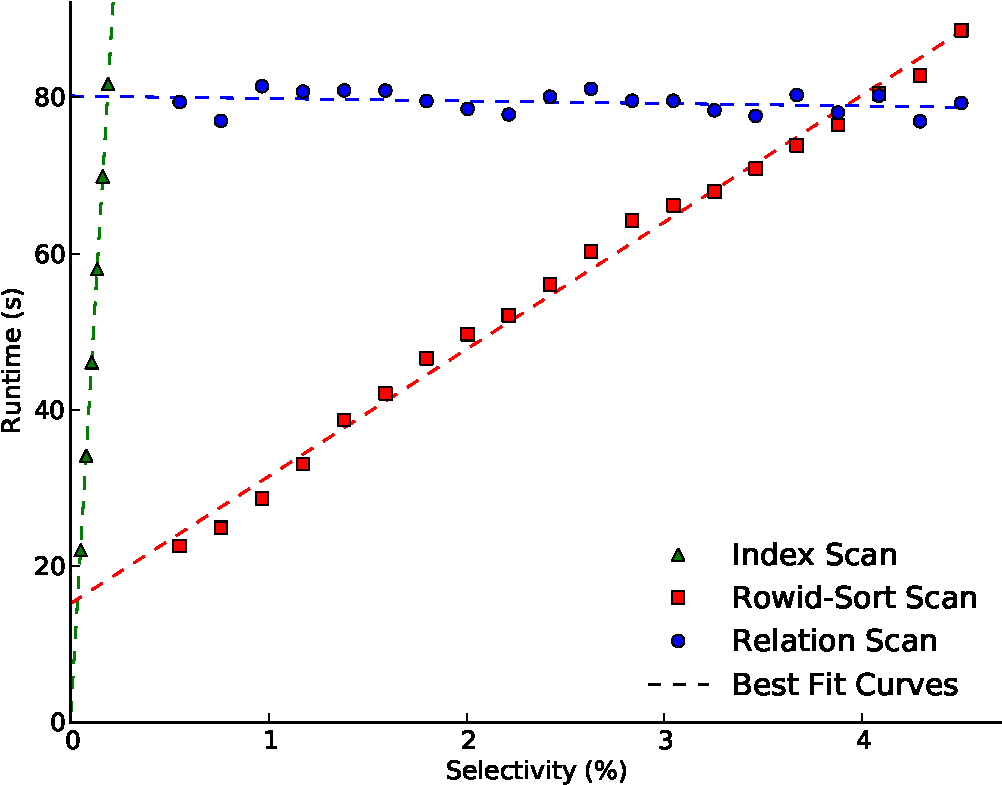
\includegraphics[width=5.0in]{FlashOpti/ScanDisk.pdf}
\caption{ \textbf{Scan operator performance on Disk.} Relation scan outperforms the alternatives at selectivities above 4\%, while index scan is optimal only for vanishingly small selectivities (e.g., single-tuple queries).  Best fit curves drawn for convenience.}
\label{fig:scan-disk}
%}
%\hspace{0.5in}
\end{figure*}
\begin{figure*}
\centering
%\subfigure[Flash SSD.]{
  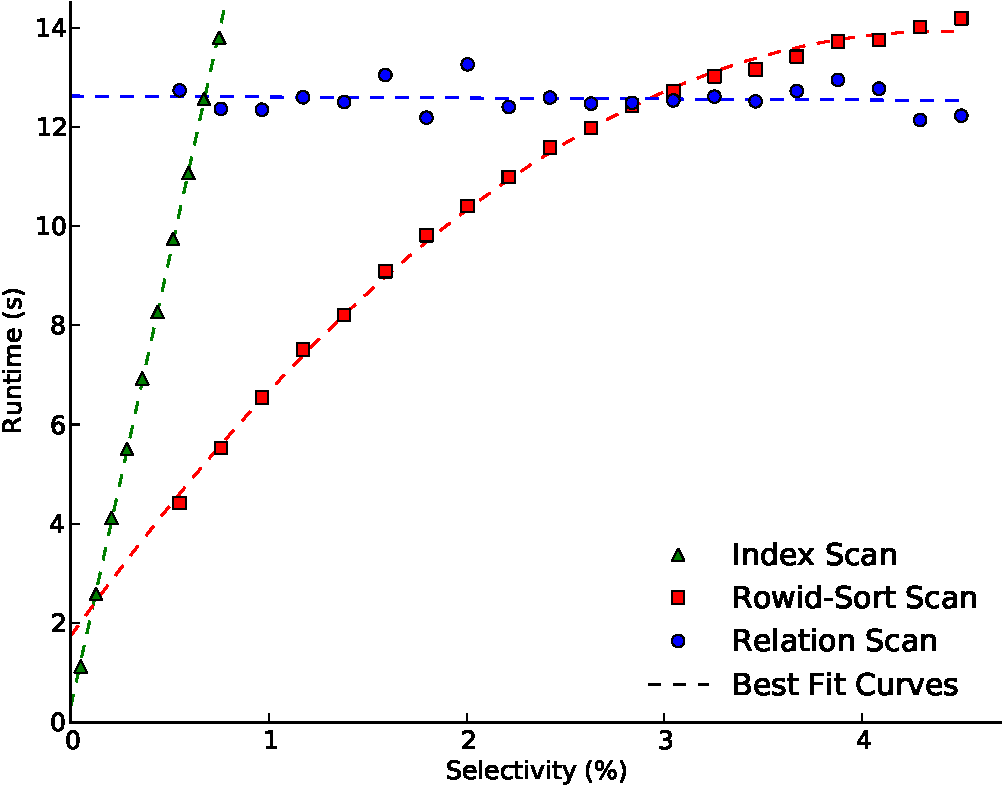
\includegraphics[width=5.0in]{FlashOpti/ScanFlash.pdf}
%}
\caption{ \textbf{Scan operator performance on Flash SSD.} Though both break-even points shift as our intuition suggests, the selectivities where the optimal decision differs between Disk and SSD are so narrow that the difference is inconsequential in practice.  Best fit curves drawn for convenience.}
\label{fig:scan-ssd}
\end{figure*}

I compare the measured performance of the different scan operators as a function of selectivity on SSD and disk.
The objective is to find the break-even points where the optimal scan operator shifts from index scan to rowid-sort scan and finally to relation scan on each device, and the performance impact in regions where this decision differs.
I issue queries for ranges of tuples using a uniformly distributed integer field on a table with 10 million rows, or roughly 2 GB. 
I use a pipelined aggregation function to ensure that no output table is materialized.

Figures~\ref{fig:scan-disk} and~\ref{fig:scan-ssd} report scan runtime on disk and Flash SSD, respectively.
The figures show the measured runtime of each scan (in seconds); lower is better. 
Recall from Section~\ref{sec:FlashOpti:Intro} that classic rules of thumb suggest that, on disk, the break-even point between index and relation scan should occur near 10\% selectivity, and intuition suggests an even higher break-even point for SSD.
Clearly, the conventional wisdom is flawed even for rotating disks; relation scan dominates above selectivities of just 4\% (the trends shown in the figure continue to the right).  
In the intermediate range from about 0.1\% to 4\% selectivity the rowid-sort scan performs best.

However, the more important analysis is to compare the locations of the break-even points across SSD and disk.  
Both crossover points shift in the expected directions.
The slope of the index scan curve is considerably shallower, and the break-even with the relation scan shifts above 0.5\% selectivity.  
Furthermore, the range in which rowid-sort scan is optimal becomes narrower.
Nevertheless, the key take-away is that the range of selectivities for which the optimal scan \emph{differs} across SSD and Disk is vanishingly small.
Only a minute fraction of queries fit into this range, and queries that make the incorrect decision (between disk and Flash) see a small performance impact.
Hence, it is unnecessary for the optimizer to be SSD-aware to choose an effective scan operation.

Whereas these measurements demonstrate my main result, they do not explain why index scans fail to leverage the random access advantage of Flash.  
I turn to this question next. 

\textbf{Analytic results.}
\begin{figure*}
\centering
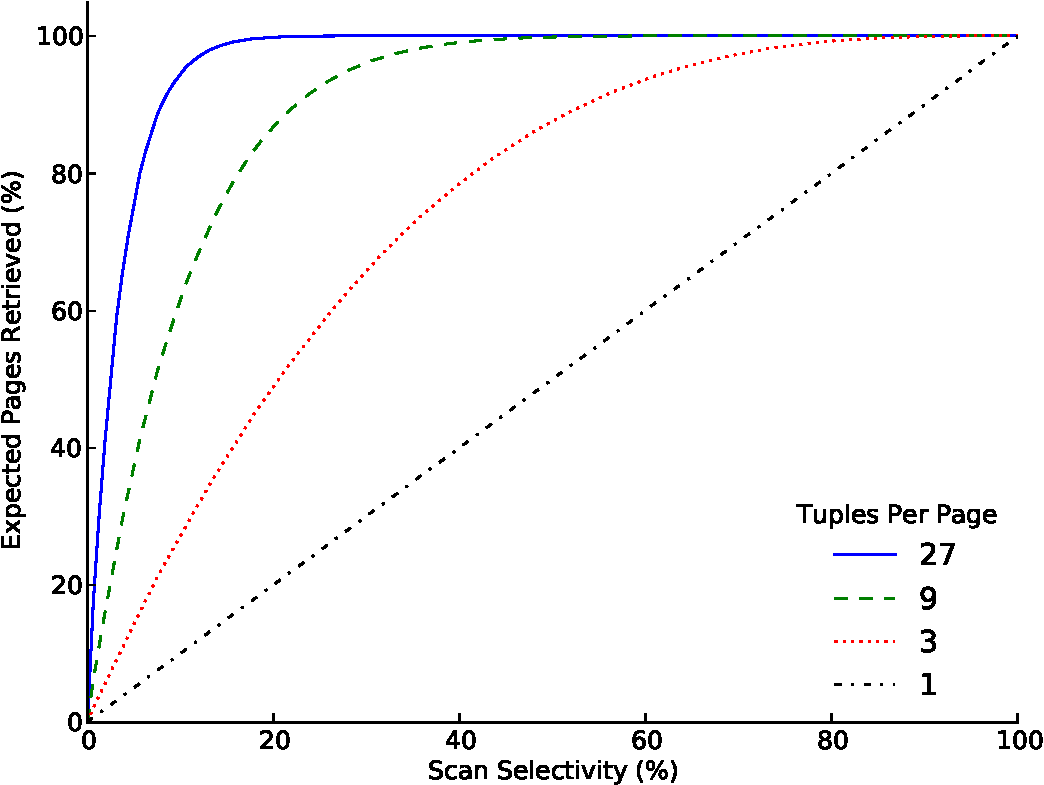
\includegraphics[width=5.0in]{FlashOpti/expectedPagesRet.pdf}
\caption{Index scans touch the majority of pages even at low selectivities.}
\label{figure::analyticScan}
\end{figure*}

The previous results show that index scan underperforms at selectivities far below what the classic 10\% rule of thumb suggests. 
The flaw in the conventional wisdom is that, when there are many tuples per page, the vast majority of \emph{pages} need to be retrieved even if only a few \emph{tuples} are accessed.
When the 10\% rule is applied to page- rather than tuple-selectivity, the guideline is more reasonable.
Yue \emph{et al.} provide an analytical formula for the expected number of pages retrieved given the size of the table, tuples per page, and selectivity \cite{Yue1975}, assuming tuples are randomly distributed among pages (a reasonable assumption given that each table can be clustered on only a single key).
Based on this formula, Figure~\ref{figure::analyticScan} shows the expected percentage of pages retrieved as a function of query selectivity and tuples per page.
When a page contains only a single tuple, clearly, the number of tuples and pages accessed are equal.
However, as the number of tuples per page increases, the expectation on the number of pages that must be retrieved quickly approaches 100\% even at small selectivities.
As a point of reference, given a 4kb page size and neglecting page headers, the Wisconsin Benchmark stores 19 tuples per page while TPC-H's Lineitem and Orders tables store 29 and 30 tuples per page, respectively.

The implication of this result is that, for typical tuple sizes, the vast majority of pages in a relation must be read even if the selectivity is but a few percent.
Hence, with the exception of single-tuple lookups, there are few real-world scenarios where scan performance improves with better random access latency under conventional storage managers that access data in large blocks.
To benefit from low access latency, future devices will need to provide random access at tuple (rather than page) granularity.
Until such devices are available, relation and rowid-sort scans will dominate, with IO bandwidth primarily determining scan performance.

\section{Join Analysis}
\label{sec:FlashOpti:Joins}

I next study the variability in join performance across disk and Flash SSD.  
Again, the objective is to identify cases where the optimal join algorithm for disk consistently results in grossly sub-optimal performance on Flash SSD.
Such scenarios imply that it is important for the optimizer to be SSD aware.

DB2 implements nested loop, sort-merge, and hybrid hash join operators.  
However, DB2 does not support a block nested loop join; its nested loop join performs the join tuple-by-tuple instead of prefetching pages or other blocks, relying on indexes to provide high performance.
Hence, unless the join can be performed in memory, the nested loop grossly underperforms the other two algorithms for ad-hoc queries (those that do not use indexes) regardless of storage device and will not be selected by the query optimizer unless it is the only alternative (e.g., for inequality joins). 
I therefore restrict the investigation to a comparison of sort-merge and hybrid hash joins.

When a clustered index exists for a particular scan or join this index should almost always be used, regardless of the nature of the storage device.  
Hence, I do not include clustered indexes in my analysis.
Furthermore, I evaluate only ad hoc joins.
When indexes are available, the choice of whether or not to use the index is analogous to the choice of which scan operator to use for a simple select query, which is covered by the previous analysis of scans.

Because of the complex interplay between available memory capacity and relation sizes for join optimization \cite{DBLP:journals/vldb/HaasCLS97}, I do not have a specific expectation that one join algorithm will universally outperform another on Flash SSD as opposed to disk.
Rather, I perform a cross-product of experiments over a spectrum of relation sizes and output projectivities using the Wisconsin Benchmark database.  
Haas's model demonstrates the importance of the relative sizes of input relations and main memory capacity on join performance; hence I explore a range of joins that are only slightly larger than available memory (joining two 1.9GB tables) to those that are an order of magnitude larger (joining two 9.7GB tables).   
I vary projectivity, having discovered empirically that it significantly impacts the optimal join algorithm on disk, as it has a strong influence on partition size in hybrid hash joins.
I execute queries with two projectivities: approximately 5\% (achieved by selecting all the integer fields in the Wisconsin Benchmark schema), and approximately 25\% (selecting an integer field and one of the three strings in the schema).
In all experiments, I perform an equijoin on an integer field, and use an aggregation operator to avoid materializing the output.

\begin{figure*}
\centering
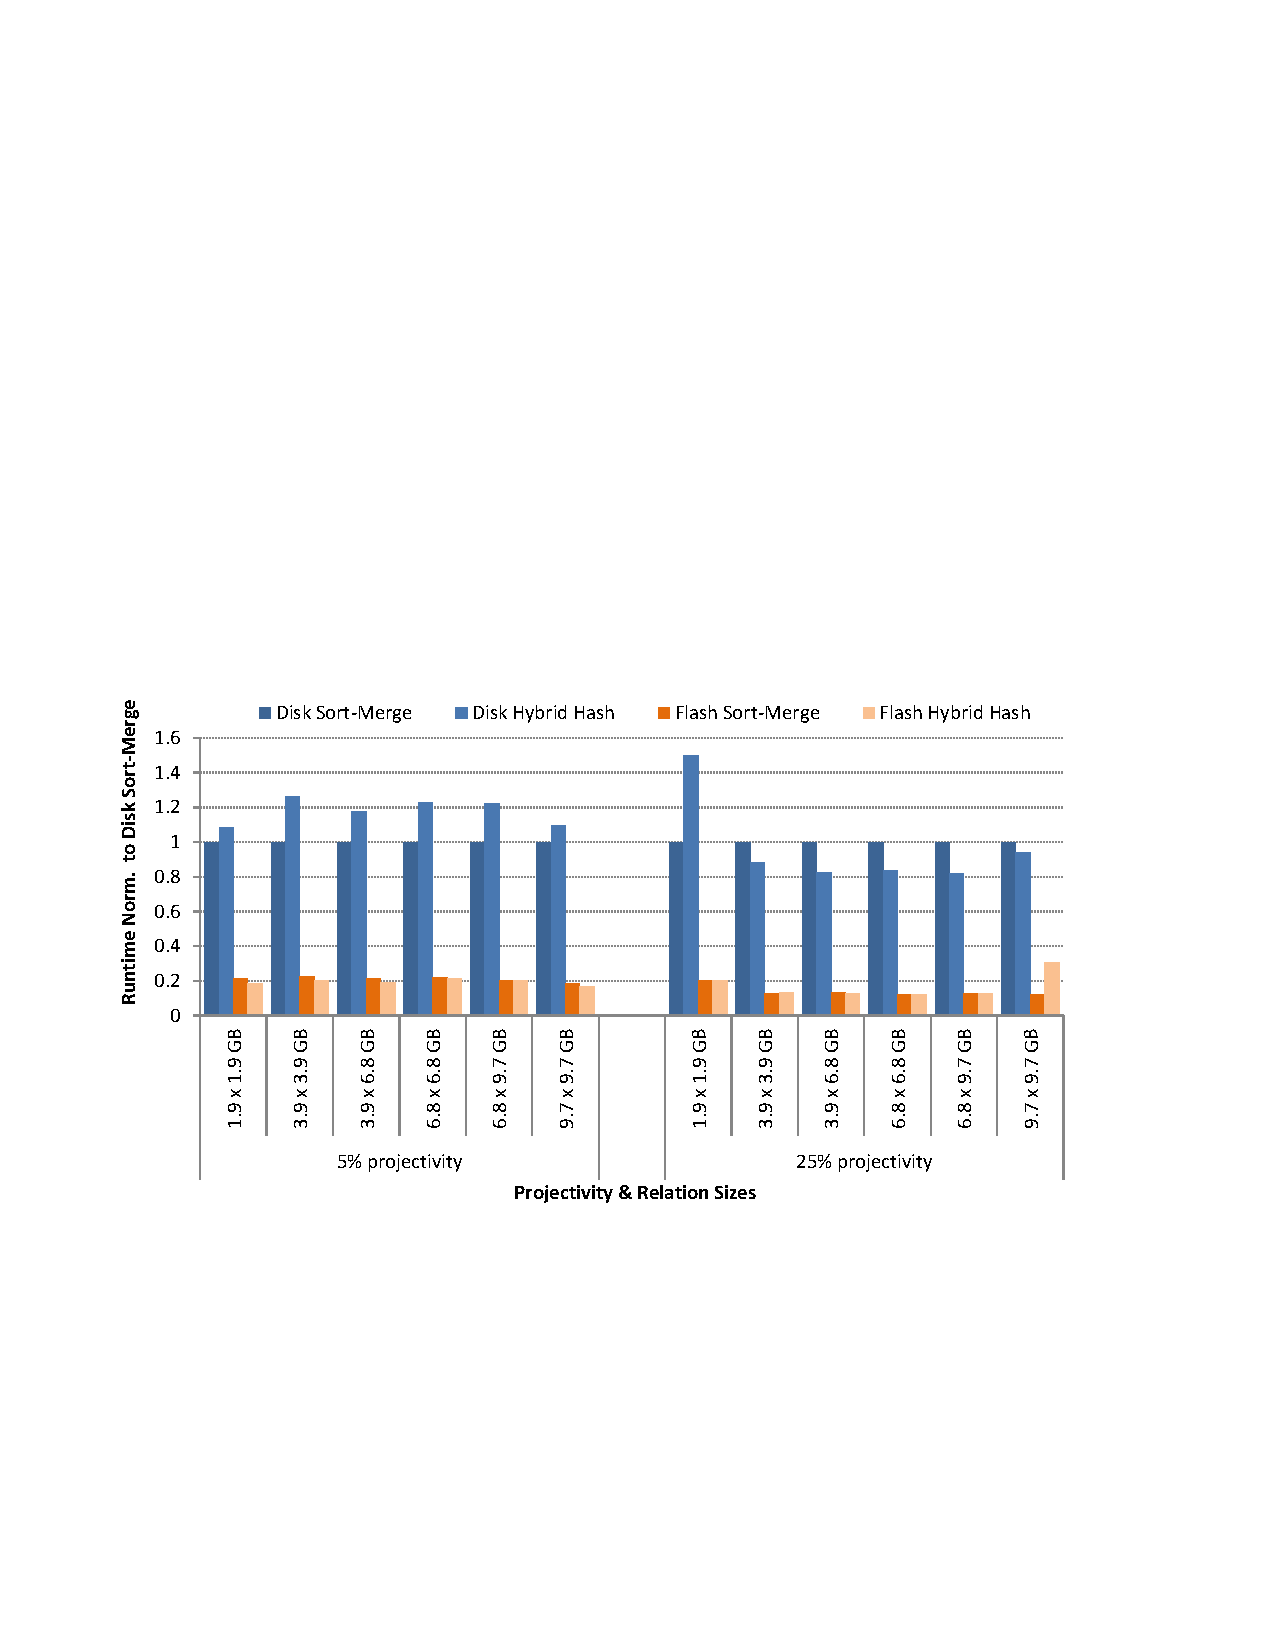
\includegraphics[width=6.0in]{FlashOpti/join.pdf}
\caption{\textbf{Join performance.}  Join runtimes on Flash SSD and Disk, normalized for each join to the runtime of sort-merge on disk.  Though there is significant variability in join algorithm performance on disk, performance variability on SSD is dwarfed by the  6\texttimes~performance advantage of moving data from disk to SSD.}
\label{figure::joins}
\end{figure*}


I report results in graphical form in Figure~\ref{figure::joins} and absolute run times in Table~\ref{table::joins}.
In Figure~\ref{figure::joins}, each group of bars shows the relative performance of sort-merge and hybrid hash joins on disk (darker bars) and Flash SSD (lighter bars), normalized to sort-merge performance on disk.
Lower bars indicate higher performance.
I provide the same data in tabular form to illustrate the runtime scaling trends with respect to relation size, which are obscured by the normalization in the graph.

Two critical results are immediately apparent from the graph.  
First, Flash SSDs typically outperform disk by 5\texttimes~to 6\texttimes~regardless of join algorithm, a margin that is substantially higher than the gap in sequential IO bandwidth, but far smaller than the gap in random IO bandwidth (see Table~\ref{table:DiskCharacteristics}).
Hence, though both join algorithms benefit from the improved random IO performance of SSDs, the benefit is muted compared to the 100\texttimes~device-level potential.
Second, whereas there is significant performance variability between the join algorithms on disk (typically over 20\%), with the exception of a single outlier, the variability is far smaller on Flash SSD (often less than 1\%).
From these results I conclude that although important on disk, the choice of sort-merge vs hybrid hash join on SSD leads to inconsequential performance differences relative to the drastic speedup of shifting data from disk to Flash.
Hence, there is no compelling reason to make the query optimizer SSD-aware; the choice it makes assuming the performance characteristics of a disk will yield near-optimal performance on SSD.

\begin{table*}
\centering
\begin{tabular}{c@{\hspace{12pt}}c@{\hspace{12pt}}c@{\hspace{12pt}}c@{\hspace{1pt}}c@{\hspace{12pt}}c@{\hspace{12pt}}c}
%\begin{tabular}{c  c | c | c | c | c}
  \toprule
	\multirow{2}{*}{Projectivity} 		      & \multirow{2}{*}{Table Sizes} & \multicolumn{2}{c}{Disk}    & &  \multicolumn{2}{c}{Flash SSD}  \\ 
\cmidrule{3-4} \cmidrule{6-7}
	 &  & Sort-merge & Hybrid hash     & &  Sort-merge & Hybrid hash  \\ 
   \midrule
5\%	& 1.9 x 1.9 GB	& 187 	& 202	& & 40		& 34	\\
	& 3.9 x 3.9 GB	& 358	& 451	& & 80		& 72	\\
	& 3.9 x 6.8 GB	& 487	& 574	& & 103	& 93	\\
	& 6.8 x 6.8 GB	& 649	& 795	& & 142	& 140\\
	& 6.8 x 9.7 GB	& 816	& 997	& & 166	& 166\\
	& 9.7 x 9.7 GB	& 1084	& 1189	& & 202	& 183\\
  \midrule
25\% & 1.9 x 1.9 GB	& 236	& 355	& & 48		& 48	\\
	& 3.9 x 3.9 GB	& 751	& 662	& & 97		& 101\\
	& 3.9 x 6.8 GB	& 947	& 781	& & 125	& 122\\
	& 6.8 x 6.8 GB	& 1415	& 1182	& & 174	& 173\\
	& 6.8 x 9.7 GB	& 1581	& 1298	& & 199	& 199\\
	& 9.7 x 9.7 GB	& 2081	& 1955	& & 250	& 634\\
  \bottomrule
\end{tabular}
\caption{\textbf{Absolute join performance.}  Join runtimes in seconds.  Variability in join runtimes is far lower on Flash SSD than on Disk.}
\label{table::joins}
\end{table*}



I highlight two notable outliers in the results.
On disk, the best join algorithm is strongly correlated to query projectivity with the exception of the 1.9GB~\texttimes~1.9GB join at 25\% projectivity.
Because the required hash table size for this join is close to the main memory capacity, I believe that this performance aberration arises due to DB2 selecting poor partition sizes for the join.
Second, on Flash, I observe a large performance difference (over 2\texttimes) between sort-merge and hybrid hash join for the largest test case, a 9.7GB~\texttimes~9.7GB join at 25\% projectivity.
For this query, I observe a long CPU-bound period with negligible IO at the end of the hybrid hash join that does not occur for any of the other hash joins.
Hence, I believe that this performance aberration is unrelated to the type of storage device, and may have arisen due to the methods employed to coax the optimizer to choose this join algorithm.
In any event, neither of these outliers outweigh the broader conclusion that there is no particular need for the query optimizer to be SSD aware.

\section{Related Work}
\label{sec:FlashOpti:RelatedWork}
Previous work studying the applicability of Flash memory in DBMS applications has focused on characterizing Flash, benchmarking specific database operations on Flash, and designing new layouts, data structures, and algorithms for use with Flash.

Both Bouganim \emph{et al.} and Chen \emph{et al.} benchmark the performance of Flash for various IO access patterns \cite{Bouganim09uflip:understanding, Chen2009}.
Bouganim introduces the uFLIP micro-benchmarks and tests their performance on several devices.
Chen introduces another set of micro-benchmarks, concluding that poor random write performance poses a significant barrier to replacing conventional hard disks with Flash SSDs.
While these micro-benchmarks are instructive for understanding database performance, I focus specifically on the performance of existing scan and join operators on SSD and disk.
Others have also benchmarked Flash's performance within the context of DBMS systems.
Lee \emph{et al.} investigate the performance of specific database operations on Flash, including multiversion concurrency control (MVCC), external sort, and hashes \cite{Lee2008}.
Similar to my study, Do \emph{et al.} benchmark ad hoc joins, testing the effects of buffer pool size and page size on performance for both disk and Flash \cite{Do2009}.
Although related to this study, neither of these works look at the specific performance differences between disk and Flash for scans and joins and how this might impact query optimization.

Whereas the above works (and this study) focus on measuring the performance of existing databases and devices, others look ahead to redesign DBMS systems in light of the characteristics of Flash.
Yin \emph{et al.} and Li \emph{et al.} present new index structures, focusing on maintaining performance while using sequential writes to update the index \cite{Yin2009, Li2009}.
Baumann \emph{et al.} investigate Flash's performance alongside a hybrid row-column store referred to as ``Grouping" \cite{Baumann2010}.
Similarly, Tsirogiannis \emph{et al.} use a column store motivated by the PAX layout to create faster scans and joins \cite{Tsirogiannis2009}.

Interestingly, my findings contradict recommendations from many of these studies.
Baumann concludes that SSDs shift optimal query execution towards index-based query plans.
The study bases this conclusion on the observation that asynchronous random reads on Flash are nearly as fast as sequential reads.
Indeed, the arguments made by Baumann are a key component of the intuition laid out in Section~\ref{sec:FlashOpti:Intro} that led me to expect a need for SSD-aware query optimization.
However, the conclusion neglects the observations discussed in Section~\ref{sec:FlashOpti:Scans} demonstrating that queries selecting more than a handful of tuples will likely retrieve the majority of pages in a relation, and thus gain no advantage from fast random IO.
Tsirogiannis introduces a join algorithm that retrieves only the join columns, joins these values, and then retrieves projected rows via a temporary index.
By the previous argument, scanning for projected data should retrieve the majority of data pages, preferring a relation scan, and thus provide comparable advantage on disk and SSD.

Finally, Bausch \emph{et al.} implement asymmetry-aware query optimization in PostgreSQL \cite{BauschPetrov12}.
They calibrate and evaluate their system using the TPC-H benchmark and find substantial improvement.
However, I believe their calibration and evaluation are skewed and lead to false conclusions (their results are insufficient to demonstrate that query optimizers should be SSD-aware).
First, their results show that an external sort of unordered data results results in 95\% random read accesses to disk.
This is indicative of poorly configured memory buffers; external soft algorithms should exhibit almost entirely sequential access patterns.
Furthermore, the results of their calibration (shown in their appendix) differ substantially from expected physical traits.
For example, the relative cost of disk's random access is only $6.8\times$ that of a sequential access, the relative cost of Flash's random read access is $5.6\times$ that of its sequential read access (nearly the same as the relative difference on disk), and Flash's sequential writes are roughly $2.5\times$ \emph{slower} than random writes (sequential writes should be faster).
Using a physically-based model only makes sense if the model is accurate.
I believe the improvement shown is a function of (1) using the total time of 21 queries as the performance and calibration metric instead of arithmetic or geometric mean (query 21 shows improvement of 549\% and has a greater runtime than most other queries), (2) using search-based calibration instead of physically derived optimization parameters (e.g., the cost of a disk seek should be measured directly from the disk, not by fitting the model), and (3) the asymmetric model has seven parameters versus the original model's five; these additional degrees of freedom allow more effective search-based calibration even when using an incorrect optimization model.
I believe that my work demonstrates fundamental principles suggesting that query optimization sees little benefit from SSD-awareness.

\section{Conclusion}
\label{sec:FlashOpti:Conclusion}
Flash-based solid state disks provide an exciting new high-performance alternative to disk drives for database applications.
My investigation of SSD-aware query optimization was motivated by a hope that the drastically improved random IO performance on SSDs would result in a large shift in optimal query plans relative to existing optimizations.
At a minimum, I expected that constants capturing relative IO costs in the optimizer would require update.
This chapter presented evidence that refutes this expectation, instead showing that an SSD-oblivious query optimizer is unlikely to make significant errors in choosing access paths or join algorithms.
Specifically, I demonstrated both empirically and analytically that the range of selectivities for which a scan operation can benefit from SSDs' fast random reads is so narrow that it is inconsequential in practice.
Moreover, measurements of alternative join algorithms reveal that their performance variability is far smaller on SSDs and is dwarfed by the 5\texttimes~to 6\texttimes~performance boost of shifting data to SSD. 
Overall, I conclude that the small and inconsistent performance gains available by making query optimizers SSD-aware are not worth the effort.


 \chapter{Architecting Recovery Management for NVRAM}
 \label{chap:OLTP_design}
 The following two chapters consider the impact of using emering NVRAM technologies for durable transaction processing.
Refer to Section~\ref{sec:Background:Storage:NVRAM} for an overview of storage technologies and Section~\ref{sec:Background:Recovery} for a description of ARIES, a popular recovery mechanism for disk.
Work relating to the next two chapters is currently under review at VLDB.
I completed this work under the advisement of my advisor, Thomas F. Wenisch, and collaborators at Oracle, Brian T. Gold and Bill Bridge.
I was the sole graduate student and technical contributer (programming and running experiments) for the project, although my co-authors were vital to development the following ideas.
I would especially like the thank Brian and Bill for bringing industry's point of view and ``real world" examples to this collaboration.

This chapter outlines the problems with existing disk recovery management, the potential pitfalls of using NVRAM for persistent applications, a methodology for evaluating NVRAM devices that do not yet exist, and a description of several candidate software designs for NVRAM recovery management, to be evaluated later.
I consider this chapter largely complete with two exceptions.
First, I have performed a validation of my timing model that has not yet been published that I intend to include in the final thesis \ref{sec:OLTP_design:Methodology:Proposed}.
Second, my implementation of \GroupCommit is more complex (and interesting, in my opinion) than a 12 page journal paper allows room to describe.
I intend to include a detailed description in Section~\ref{sec::OLTP_design:GroupCommit:Proposed}.

\section{Introduction}
\label{sec:OLTP_design:Intro}

Emerging nonvolatile memory technologies (NVRAM) offer an alternative to disk that is persistent, provides read latency similar to DRAM, and is byte-addressable \cite{BurrKurdi08}.
Such NVRAMs could revolutionize online transaction processing (OLTP), which today must employ sophisticated optimizations with substantial software overheads to overcome the long latency and poor random access performance of disk.
Nevertheless, many candidate NVRAM technologies exhibit their own limitations, such as greater-than-DRAM latency, particularly for writes \cite{LeeIpek09}.

These NVRAM technologies stand to revolutionize Online Transaction Processing (OLTP), where consistency and durability are paramount, but applications demand high throughput and low latency.
Prior work has already demonstrated the potential of these technologies to enhance file systems \cite{GreenanMiller06, ConditNightingale09} and persistent data structures \cite{VenkataramanTolia11}, but has not considered OLTP. 
Today, OLTP systems are designed from the ground up to circumvent disk's performance limitations.
For example, many popular database systems use Write-Ahead Logging (WAL; e.g., ARIES \cite{MohanHaderle92}) to avoid expensive random disk writes by instead writing to a sequential log.  
Although effective at hiding write latency, WAL entails substantial software overheads.

NVRAM offers an opportunity to simultaneously improve database forward-processing throughput and recovery latency by rethinking mechanisms that were designed to address the limitations of disk.
Figure~\ref{fig::Recovery} demonstrates this potential, displaying recovery time and transaction throughput for the TPCB workload running on the Shore-MT storage manager \cite{JohnsonPandis09} for hypothetical NVRAM devices (see Section~\ref{sec:OLTP_design:Methodology} for a description of the methodology).

\begin{figure}
  \centering
  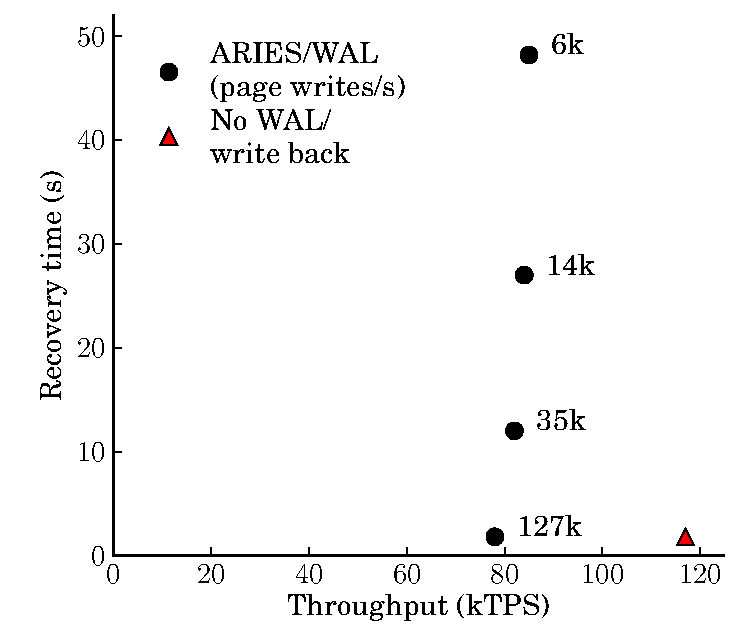
\includegraphics[width=.6\linewidth]{OLTP_design/TPCB_Recovery.pdf}
  \caption{\textbf{TPCB recovery latency vs throughput.} Increasing page flush rate reduces recovery latency.  Removing WAL entirely improves throughput by 50\%.}
  \label{fig::Recovery}
\end{figure}


The ARIES/WAL points (black circles) in the Figure show forward-processing throughput (horizontal axis) and recovery time (vertical axis) as a function of device write throughput (annotated alongside each point).
As database throughput can greatly outpace existing storage devices (this configuration requires 6,000 page writes/s to bound recovery at maximum transaction throughput; measured disk and flash devices provide only 190 and 2,500 page writes/s, respectively) I model recovery performance under faster NVRAM using a RAM disk for log and store while limiting the page flush rate.
As intuition would suggest, greater write bandwidth enables more aggressive flushing, minimizing the number of dirtied pages in the buffer cache at the time of failure, reducing recovery time.
With enough write bandwidth (in this case, 127,000 flushes/s, or 0.97 GB/s random writes for 8KB pages) the database recovers near-instantly, but forward-processing performance remains compute bound.
Achieving such throughput today requires large, expensive disk arrays or enterprise flash storage devices; future NVRAM devices might enable similar performance on commodity systems.

NVRAM opens up even more exciting opportunities for recovery management if we consider re-architecting database software.
The Figure shows this additional potential with a design point (red triangle) that removes WAL and asynchronous page flushing---optimizations primarily designed to hide disk latency.
Throughput improves due to three effects: (1) threads previously occupied by page and log flushers become available to serve additional transactions, (2) asynchronous page flushing, which interferes with transactions as both flusher and transaction threads latch frequently accessed pages, is removed, and (3) transactions no longer insert WAL log entries, reducing the transaction code path.
In aggregate these simplifications amount to a 50\% throughput increase over ARIES's best possible NVRAM performance.
The key take-away is that database optimizations long used for disk only hinder performance with faster devices.
In this chapter, I investigate how to redesign durable storage and recovery management for OLTP to take advantage of the low latency and byte-addressability of NVRAM.

NVRAMs, however, are not without their limitations.
Se\-veral candidate NVRAM technologies exhibit larger read latency and significantly larger write latency compared to DRAM.
Additionally, whereas DRAM writes benefit from caching and typically are not on applications' critical paths, NVRAM writes must become persistent in a constrained order to ensure correct recovery.
I consider an NVRAM access model where correct ordering of persistent writes is enforced via \emph{persist barriers}, which stall until preceding NVRAM writes are complete; such persist barriers can introduce substantial delays when NVRAM writes are slow.

This chapter outlines an approach to architecting recovery management for transaction processing using NVRAM technologies
I discuss potential performance problems with using NVRAM and possible software architectures to address these problems.
Additionally, I propose an evaluation framework, involving memory trace analysis, code annotation, and precise timing models for OLTP running on existing hardware platforms.
Subsequent chapters will build on the designs and methodology presented here to determine when OLTP must be redesigned and what problems might remain.

\section{Recovery Management Design}
\label{sec:OLTP_design:Design}

\begin{table*}
  \footnotesize
  \centering
  \renewcommand{\arraystretch}{2.5}
  \begin{tabular*}{\textwidth}{l l l l}
     & \pbox{1.1 in}{\emph{NVRAM\newline Disk-Replacement}} & \pbox{1.5 in}{\InPlace} & \pbox{1.5 in}{\GroupCommit} \\
    \emph{Software buffer} & \cellcolor[gray]{.8}\pbox{1.1 in}{Traditional WAL/ARIES} & \cellcolor[gray]{.8}\pbox{1.5 in}{Updates both buffer and NVRAM} & \cellcolor[gray]{.8}\pbox{1.5 in}{Buffer limits batch size} \\
    \emph{Hardware buffer} & \cellcolor[gray]{.95}\pbox{1.1 in}{Impractical} & \cellcolor[gray]{.95}\pbox{1.5 in}{Slow uncached NV\-RAM reads} & \cellcolor[gray]{.95}\pbox{1.5 in}{Requires hardware support} \\
    \emph{Replicate to DRAM} & \multicolumn{3}{l}{\pbox{4.1 in}{\cellcolor[gray]{.8}Provides fast reads and removes buffer management, but requires large DRAM capacity}} \\
  \end{tabular*}
  \caption{\textbf{NVRAM design space.} Database designs include recovery mechanisms (top) and cache configurations (left).}
  \label{table::DesignSpace}
\end{table*}


Near-future NVRAM devices will undoubtedly be faster than both disk and flash.
However, compared to DRAM many NVRAM technologies impose slower reads and significantly slower persistent writes.
We must consider both in redesigning OLTP for NVRAM.

\subsection{NVRAM Reads}
\label{sect:OLTP_design:Design:Reads}
While the exact read performance of future NVRAM technologies is uncertain, many technologies and devices increase read latency relative to DRAM.
Current databases and computer systems are not equipped to deal with this read latency.
Disk-backed databases incur sufficiently large read penalties (on the order of milli-seconds) to justify software-managed DRAM caches and buffer management.
On the other hand, main-memory databases rely only on the DRAM memory system, including on-chip data caches.
Increased memory latency and wide-spread data accesses may require hardware or software-controlled DRAM caches even when using byte addressable NVRAM.

I consider three configurations of cache management; these alternatives form the three rows of Table~\ref{table::DesignSpace} (subsequent sections consider the recovery management strategies, forming the three columns).
The first option, \emph{Software Buffer}, relies solely on software to manage a DRAM buffer cache, as in conventional disk-backed database systems.
The cache may be removed entirely or execution relies soly on a \emph{Hardware Buffer}, as in main-memory databases.
Hardware caches are fast (e.g., on-chip SRAM) and remove complexity from the software, but provide only limited capacity.
Third, one might \emph{replicate to DRAM} all data that is stored in NVRAM---all writes update both DRAM and NVRAM (for recovery), but reads retrieve data exclusively from DRAM.
Replicating data ensures fast reads by avoiding increased NVRAM read latencies (except for recovery) and simplifies buffer management, but requires large DRAM capacity.

\subsection{NVRAM Writes}
\label{sec:OLTP_design:Design:Writes}

Persistent writes, unlike reads, do not benefit from cach\-ing; writes persist through to the device for recovery correctness.
Additionally, NVRAM updates must be carefully ordered to ensure consistent recovery.
I assume that ordering is enforced through a generic mechanism called a \emph{persist barrier}, which guarantees that writes before the barrier persist before any dependant operations after the barrier persist.

Persist barriers may be implemented in several ways.
The easiest, but worst performing, is to delay threads that issue persist barriers until all pending NVRAM writes successfully persist.
More complicated mechanisms improve performance by allowing threads to continue executing beyond the persist barrier and only delaying thread execution when persist conflicts arise (i.e., a thread reads or overwrites shared data from another thread that has not yet persisted).
BPFS provides an example implementation of this mechanism \cite{ConditNightingale09}.
Regardless of how they are implemented, persist barriers can introduce expensive synchronous delays on transaction threads; the optimal recovery mechanism depends on how expensive, on average, persist barriers become.
To better understand how persist barriers are used and how frequently they occur, I outline operations to atomically update persistent data using persist barriers, and use these operations to implement three recovery mechanisms for NVRAM.

\textbf{Atomic durable updates.}
{
\singlespacing
\newsavebox{\persistwal}
\begin{lrbox}{\persistwal}
\begin{lstlisting}
persist_wal(log_buffer, nvram_log)
  for entry in log_buffer:
    nvram_log.force_last_lsn_invalid(entry)
    nvram_log.insert_body(entry) # no lsn
  persist_barrier()
  nvram_log.update_lsns()
  persist_barrier()
\end{lstlisting}
\end{lrbox}

\newsavebox{\persistpage}
\begin{lrbox}{\persistpage}
\begin{lstlisting}
persist_page(page_v, page_nv, page_log)
  page_log.copy_from(page_nv)
  persist_barrier()
  page_log.mark_valid()
  persist_barrier()
  page_nv.copy_from(page_v)
  persist_barrier()
  page_log.mark_invalid()
  persist_barrier()
\end{lstlisting}
\end{lrbox}

\begin{figure}[]
  \subfigure{ \usebox{\persistwal} }
  \subfigure{ \usebox{\persistpage} }

  \caption{\textbf{Durable atomic updates.} \texttt{persist\_wal()} appends to the ARIES log using two persist barriers.  \texttt{persist\_page()} persists pages with four persist barriers.}
  \label{fig::Code}
\end{figure}
}

Figure~\ref{fig::Code} shows two operations to atomically update NVRAM data.
The first, \texttt{persist\_wal()}, persists log entries into an ARIES log.
Sho\-re-MT log entries are post-pended with their Log Serial Number (LSN -- log entry file offset).
At recovery, a log entry is considered valid only if this tail LSN matches the location of the entry.
I persist log entries atomically by first persisting an entry without its tail LSN, and only later (once we are certain the entry is persistent) persist the LSN.
This order is enforced by inserting a persist barrier between writing the log entry and its LSN.
Additionally, I reduce the number of persist barriers by persisting entries in batches, writing several log entries at once (without LSNs), followed by all their LSNs, separated by a single persist barrier.
It is entirely possible (yet unlikely) that pre-existing LSN tails already match the log entry's offset; tails must be checked and first reset when this occurs.
Log operations introduce two persist barriers---one to ensure that log entries persist before their LSNs, and one to enforce that LSNs persist before the thread continues executing.

The second operation, \texttt{persist\_page()}, atomically persists page data with the use of a persistent undo page log.
First, the page's original data is copied from NVRAM to the page log.
The page log is marked valid and the dirty version of the page is copied to NVRAM (or updated in-place while locks are held).
Finally, the log is marked invalid.
Four persist barriers ensure that each update persists before the next, enforcing consistency at all points in execution.
Recovery checks the valid flags of all page logs, copying any valid log back in-place.
The log is always valid while the page persists in-place, protecting against partial NVRAM writes.
Together, \texttt{persist\_wal()} and \texttt{persist\_page()} provide the tools necessary to construct recovery mechanisms.
I discuss these mechanisms next, describing their implementation and performance.

\textbf{NVRAM Disk-Replacement.}
NVRAM database systems will likely continue to rely on ARIES/WAL at first, using NVRAM as \NVDisk.
WAL provides recovery for disk by keeping an ordered log of all updates, as described in Section~\ref{sec:Background:Recovery}.
While retaining disk's software interface, NVRAM disk accesses are implemented as copies between the volatile and nonvolatile address spaces.
\NVDisk in Shore-MT persists the log and pages with \texttt{persist\_wal()} and \texttt{persist\_page()}, respectively.
However, persists occur on log and page flusher threads, and transaction threads do not observe persist barrier delays (except when waiting for commit log entries to persist).
\NVDisk provides low recovery latency by aggressively flushing pages, minimizing the size of data to recover.
While requiring the least engineering effort, \NVDisk contains large software overheads to maintain a centralized log and asynchronously flush pages.
Next, I leverage NVRAM's low latency to reduce these overheads.

\textbf{In-Place Updates.}
Fast, byte-addressable NVRAM allows updates to persist in-place and enforce persist order immediately, a design we call \InPlace.
\InPlace allows us to remove the centralized log by replacing redo and undo log functionality elsewhere.
I remove redo logs by keeping the database's durable state up-to-date.
In ARIES terms, the database is constantly at its replayed state---there is no need to replay a redo log after failure.
Undo logs need not maintain a global order (transactions are already free to roll back in any order), and instead I distribute ARIES undo logs per transaction.
Such non-concurrent logs are simpler and impose less overhead than centralized logs.
Other databases (such as Oracle) already distribute undo logs in rollback segments and undo table spaces \cite{OracleDoc}.
Transaction undo logs remain durable so that in-flight transactions at the time of failure can be rolled back.
Each page update consists of (1) latching the page, (2) inserting an undo entry into the transaction-private undo log, using \texttt{persist\_wal()}, (3) updating the page in-place, using \texttt{persist\_page()} (without an intermediate volatile page), and (4) releasing the page latch.
This protocol ensures all updates to a page, and updates within a transaction, persist in-order, and that no transaction reads data from a page until it is durable.
Recovery applies undo logs for in-flight transactions; there is no need to replay a redo log.

Persisting data in-place removes expensive redo logging and asynchronous page flushing, but introduces persist barriers on transactions' critical paths.
For sufficiently short persist barrier delays \InPlace outperforms \NVDisk (if persist barrier delays are negligible \InPlace resembles existing non-recoverable in-memory databases).
However, one would expect transaction performance to suffer as persist barrier delay increases.

In response, I introduce \GroupCommit, a recovery mechanisms designed to minimize the frequency of persist barriers while still removing WAL.
\GroupCommit is an entirely new design, committing instructions in large batches to minimize persist synchronization.
The next section describes, in detail, the operation and data structures necessary to implement \GroupCommit.

\section{NVRAM Group Commit}
\label{sec:OLTP_design:GroupCommit}

The two previous recovery mechanisms provide high throughput under certain circumstances, but also fail to perform in others.
\NVDisk is insensitive to large persist barrier delays as it was originally designed for disk.
However, it assumes IO delays to be the dominant performance bottleneck and trades off software overhead to minimize IO.
\InPlace, on the other hand, excels when persist barriers delays are short.
As persist barrier latency increases performance suffers, such that \NVDisk eventually performs better.
Here, I provide a third option, coupling \NVDisk's persist barrier latency-insensitivity with \InPlace's low software overhead: \GroupCommit.

\subsection{Operating Principles and Implementation}
\label{sec:OLTP_design:GroupCommit:Proposed}

\GroupCommit operates by executing transactions in batches, whereby all transactions in the batch commit or (on failure) all transactions abort.
Transactions quiesce between batches, allowing only transactions from the oldest batch to execute.
Each transaction maintains a private ARIES-style undo log, supporting abort and roll-back as in \InPlace, but transaction logs are no longer persistent.
ARIES undo logs support concurrent durable transactions.
As batches persist atomically, transactions no longer roll back selectively during recovery, obviating the need for persistent ARIES undo logs.
Instead, recovery relies on a database-wide undo log and staging buffer to provide durable atomic batches.

\GroupCommit limits persist barrier frequen\-cy by enforcing persistence by batch rather than by transaction.
Persisting a batch resembles \texttt{persist\_page()}, used across the entire database, once per batch.
Because undo logging is managed at the batch level, transactions' updates may not persist in-place to NVRAM until all transactions in the batch complete.
Rather, transactions write to a volatile staging buffer, tracking dirtied cache lines in a concurrent bit field.
The bit field facilities quickly finding all dirtied data at batch completion.
Once the batch ends and all transactions complete, the pre-batch version of dirtied data is copied to the database-wide persistent undo log, only after which is data copied from the staging buffer in-place to NVRAM.
Finally, the database-wide undo log is invalidated, transactions commit, and transactions from the next batch begin executing.
%Batching allows NVRAM persists to coalesce -- the log persists only the earliest version of data from the batch, while only the last version of data persists in-place, with intermediate values never persisting.
On failure the log is copied back to the NVRAM database, aborting and rolling back all transactions from the in-flight batch.
The key observation is that \GroupCommit persists entire batches of transactions using four persist barriers, far fewer than required with \InPlace.  Note, however, that it enables recovery only to batch boundaries, rather than transaction boundaries.

I briefly outline two implementation challenges: long transactions and limited staging buffers.
Long transactions present a problem by forcing all other transactions in the batch to defer committing until the long transaction completes.
Limited staging buffers, not large enough to fit the entire data set, may fill while transactions are still executing.
I solve both problems by resorting to persistent ARIES-style undo logs, as in \InPlace.
Long transactions persist their ARIES undo log (previously volatile), allowing the remainder of the batch to persist and commit.
The long transaction joins the next batch, committing when that batch commits.
At recovery the most recent batch rolls back, and the long transaction's ARIES undo log is applied, removing updates that persisted with previous batches.
Similarly, if the staging buffer fills, the current batch ends immediately and all outstanding transactions persist their ARIES undo logs.
The batch persists, treating any in-flight transactions as long transactions, reassigning them to the next batch.
Transaction-local ARIES undo logs invalidate as the batch commits, requiring additional persistent data structures to allow transaction and batch logs to invalidate atomically.

\GroupCommit requires fewer persist barriers than \InPlace yet avoids expensive logging found in \NVDisk.
A batch requires only four persist barriers, regardless of batch length.
Expensive persist barrier delays can be amortized over additional transactions by increasing batch length, improving throughput.
Batch length must be at least large enough to amortize time spent quiescing transactions between batches.
However, increasing batch length defers commit for all transactions in the batch, increasing transaction latency.

\subsection{Proposed Work}
\label{sec::OLTP_design:GroupCommit:Proposed}

\GroupCommit only improves throughput so long as the time between batches to quiesce transactions, locate dirtied data, and persist that data is substantially less than time during each batch where transactions execute.
To provide a fair comparison between recovery mechanisms, I implement a true version of \GroupCommit in Shore-MT.
Whereas I expect NVRAM to have sufficient bandwidth to persist data quickly, orchestrating data copies, tracking dirty data with low overhead, and locating dirty data efficiently proved to be difficult software problems.
The details of this implementation were omitted from the VLDB submission, but are included here, including work to be done.

\textbf{Concurrent Dirty Set.}
As described previously, \GroupCommit requires each batch to track dirty data.
This is done with an efficient concurrent set, tracking the set of buffer pool cache lines dirtied by each batch.
In order to maximize transaction throughput, this set must allow low overhead updates by concurrent threads during batch execution, and fast iteration during batch persist.

The first attempt to create a set used an STL \emph{ordered\_set} (implemented as a balanced tree).
However, inserting cache lines to the dirty set was prohibitively expensive, slowing transactions down.
On the other hand, \emph{ordered\_set} allows relatively fast iteration over the dirty set during batch copy.
The next attempt used a bitmap of dirty cache lines, each bit corresponding to a cache line in the buffer pool.
A 10GB buffer pool requires 20MB of bits to track dirty cache lines.
Before each batch starts, after the previous batch finishes persisting, dirty bits must be flash cleared in order to track the next batch.
While bits can be quickly updated via an atomic OR operation, iterating over the dirty bits during persist was too slow, requiring a different solution.

Instead, I leveraged the fact that dirty regions were rare and sparsely located throughput the buffer pool.
Batches contain up to thousands of transactions, yet these transactions could only manage to write to a small portion of a 10GB buffer pool.
It is therefore necessary to efficiently skip over large regions of clean data when iterating through the dirty set.
To achieve this, I created a \emph{tiered bitfield set}.
The tiered bitfield set contains two bitfield sets.
The first is as described above, where each bit corresponds to a cache line in the buffer pool.
In addition, there is a higher level bit field, each bit corresponding to a \emph{cache line of the primary bit field}.
Thus, a set bit in the top level bit field indicates that some bit within a cache line of the primary bit field is set, which in turn corresponds to dirty cache line in the buffer pool.

Updating this set requires atomic OR on the necessary bits in both bit fields of the set, a small cost.
Iterating over the set now involves iterating over the (much smaller) top level bit field, finding \emph{segments} of the primary bit field known to contain at least one set bit.
This iteration reduces both the number of instructions and cache/memory lines accessed, minimizing persist time between batches.

I propose to include additional work demonstrating the sparse nature of writes to the buffer pool, as well as timing results that show that fast dirty line tracking and persist is possible.

\textbf{Concurrent Persist.}
I have shown that dirty lines can be tracked and iterated over efficiently.
However, persisting each batch with the batch coordinator alone results in long persist delays.
These delays are due to the \emph{software} overhead of copying data, not from NVRAM limitations.
To reduce these delays all persist operations must be parallelized across threads.
Luckily, we have threads to spare -- transaction threads that have quiesced between batches.
Instead of sitting idle, these threads now participate in persisting each batch.

The buffer pool address space and corresponding portions of the dirty line set are partitioned into several segments, each placed in a task queue.
The batch coordinator and transaction threads blocked by the persist process each participate by accepting tasks to persist buffer pool partitions (both log and then data in-place).
Once all tasks complete the batch commits, allowing the next batch to begin.

I propose to include results showing that persist parallelization is necessary, but is an effective way to accelerate batching.

Once both of these optimizations are implemented the system is using all cores to persist, and profiling shows that \emph{memcpy} operations, copies from the buffer pool to the persistent address space, are the primary bottleneck (memcpy is implemented using fast SSE instructions and cannot be optimized further).
Persist time is minimized, and there is little room left for improvement.

\section{Design Space}
\label{sec:OLTP_design:Designs}
I describe the space of possible designs given choices regarding NVRAM read and write performance.
This discussion ignores possible uses of hard disk to provide additional capacity.
Each design works alongside magnetic disk with additional buffer management and the constraint that pages persist to disk before eviction from NVRAM.

Table~\ref{table::DesignSpace} lists the possible combinations of caching architectures and recovery mechanisms.
The left column presents \NVDisk, which we see as the obvious and most incremental use for NVRAM.
Of note is the center-left cell, \NVDisk without the use of a volatile buffer.
WAL, by its design, allows pages to write back asynchronously from volatile storage.
Removing the volatile cache requires transactions to persist data in-place, but do so only after associated log entries persist, retaining the software overheads of \NVDisk as well as the frequent synchronization in \InPlace.
Thus, this design is impractical.

The middle-column recovery mechanism, \InPlace, represents the most intuitive use of NVRAM in database systems, as noted in several prior works.
Agrawal and Jagadish explore several algorithms for atomic durable transactions with an NVRAM main-memory \cite{AgrawalJagadish89}.
They describe the operation and correctness of each mechanism and provide an analytic cost model to compare them.
Their work represents the middle column, middle row of Table~\ref{table::DesignSpace} (\InPlace with no volatile buffer).
Aky\"{u}rek and Salem present a hybrid DRAM and NVRAM buffer cache design alongside strategies for managing cache allocation \cite{SalemAkyrek95}.
They evaluate their allocation strategies using database traces and queuing models to demonstrate the effectiveness of NVRAM at accelerating persistent writes.
Partial Memory Buffers is closest to the middle-top cell of the design space table (\InPlace with a software-managed DRAM buffer), although that design considers NVRAM as part of a hybrid buffer, not the primary persistent store.
None of these works considers alternative approaches (such as \GroupCommit), to account for large persist barrier latency and associated delays.
Additionally, This work extends prior work by providing a more precise performance evaluation and more detailed consideration of NVRAM characteristics.

The right column presents \GroupCommit.
I am not aware of any previous work that extends disk group commit to reduce the frequency of NVRAM persist barriers.
A limited-capacity staging buffer (i.e., one insufficient for the entire data set) may limit batch size, as described above.

Each of the three recovery mechanisms may replicate all data between NVRAM and DRAM to ensure fast read accesses, manage a smaller DRAM buffer cache, or omit the cache altogether.
In Section~\ref{sec:OLTP_eval:Reads} I consider the importance of NVRAM caching to transaction throughput.
Then, in Section~\ref{sec:OLTP_eval:Persists} I assume a DRAM-replicated data store to isolate read performance from persist performance in evaluating each recovery mechanisms's ability to maximize transaction throughput.
The next section describes an evaluation methodology for OLTP on NVRAM.

\section{Methodology}
\label{sec:OLTP_design:Methodology}

This section details the methodology for benchmarking transaction processing and modeling NVRAM performance.
Experiments use the Shore-MT storage manager \cite{JohnsonPandis09}, including the high performance, scalable WAL implementation provided by Aether \cite{JohnsonPandis10}.
While Aether provides a distributed log suitable for multi-socket servers, the distributed log exists as a fork of the main Shore-MT project.
Instead, I limit experiments to a single CPU socket to provide a fair comparison between WAL and other recovery schemes, enforced using the Linux \emph{taskset} utility.
Experiments place both the Shore-MT log and volume files on an in-memory \emph{tmpfs}, and provide sufficiently large buffer caches such that all pages hit in the cache after warmup.
The intent is to allow the database to perform data accesses at DRAM speed and introduce additional delays to model NVRAM performance.
Table~\ref{table::Specs} shows the experimental system configuration.

\begin{table}
  \centering
  \begin{tabular}{l l}
    \hline
    Operating System & Ubuntu 12.04 \\
    CPU & Intel Xeon E5645 \\
    & 2.40 GHz \\
    CPU cores & 6 (12 with HyperThreading) \\
    Memory & 32 GB \\
    \hline
  \end{tabular}
  \caption{\textbf{Experimental system configuration.}}
  \label{table::Specs}
\end{table}

\textbf{Modeling NVRAM delays.}
Since NVRAM devices are not yet available, we must provide a timing model that mimics their expected performance characteristics.
I model NVRAM read and write delays by instrumenting Shore-MT with precisely controlled assembly-code delay loops to model additional NVRAM latency and bandwidth constraints at 20ns precision.
Hence, Shore-MT runs in real time as if its buffer cache resided in NVRAM with the desired read and write characteristics.

I introduce NVRAM read and write delays separately.
Accurately modeling per-access increases in read latency is challenging, as reads are frequent and the expected latency increases on NVRAM are small.
It is infeasible to use software instrumentation to model such latency increases at the granularity of individual reads; hardware support, substantial time dilation, or alternative evaluation techniques (e.g., simulation) would be required, all of which compromise accuracy and the ability to run experiments at full scale.
Instead, I use offline analysis with PIN \cite{LukCohn05} to determine (1) the reuse statistics of buffer cache pages, and (2) the average number of cache lines accessed each time a page is latched.
Together, these offline statistics provide an average number of cache line accesses per page latch event in Shore-MT while considering the effects of page caching.
I then introduce a delay at each latch based on the measured average number of misses and an assumed per-read latency increase based on the NVRAM technology.

I model NVRAM persist delays by annotating Shore-MT to track buffer cache writes at cache line granularity---64 bytes---using efficient ``dirty" bitmaps.
Depending on the recovery mechanism, we introduce delays corresponding to persist barriers and to model NVRAM write bandwidth contention.
Tracking buffer cache writes introduces less than a 3\% overhead to the highest throughput experiments.

I create NVRAM delays using the x86 RDTSCP instruction, which returns a CPU-frequency-invariant, monotonically increasing time-stamp that increments each clock tick.
RDTSCP is a synchronous instruction---it does not allow other instructions to reorder with it.
The RDTSCP loop delays threads in increments of 20ns (latency per loop iteration and RDTSCP) with an accuracy of 2ns.

In addition to NVRAM latency, I model shared NVRAM write bandwidth.
Using RDTSCP as a clock source, I maintain a shared \emph{next\_available} variable, representing the next clock tick in which the NVRAM device is available to be written.
Each NVRAM persist advances \emph{next\_available} to account for the latency of its persist operation.
Reservations take the maximum of \emph{next\_available} and the current RDTSCP and add the reservation duration.
The new value is atomically swapped into \emph{next\_available} via a Compare-And-Swap (CAS).
If the CAS fails (due to a race with a persist operation on another thread), the process repeats until it succeeds.
Upon success, the thread delays until the end of its reservation.
The main limitation of this approach is that it cannot model reservations shorter than the delay required to perform a CAS to a contended shared variable.
This technique models reservations above 85ns accurately, which is sufficient for my experiments.

I choose on-line timing modeling via software instrumentation in lieu of architectural simulations to allow experiments to execute at full scale and in real time.
While modeling aspects of NVRAM systems such as cache performance and more precise persist barrier delays require detailed hardware simulation, I believe NVRAM device and memory system design are not sufficiently established to consider this level of detail.
Instead, I investigate more general trends to determine if and when NVRAM read and write performance warrant storage management redesign.

\textbf{Recovery performance.} Figure~\ref{fig::Recovery} displays recovery latency vs transaction throughput for the TPCB workload, varying page flush rate.
Page flush rate is controlled by maintaining a constant number of dirty pages in the buffer cache, always flushing the page with the oldest volatile update.
Experiments run TPCB for one minute (sufficient to reach steady state behavior) and then kill the Shore-MT process.
Before starting recovery I drop the file system cache.
Reported recovery time includes only the recovery portion of the Shore-MT process; I do not include system startup time nor non-recovery Shore-MT startup time.

\textbf{Workloads}
I use three workloads and transactions in this evaluation: TPCC, TPCB, and TATP.
TPCC models order management for a company providing a product or service \cite{TPCC}.
TPCB contains one transaction class and models a bank executing transactions across branches, tellers, customers, and accounts \cite{TPCB}.
TATP includes seven transactions to model a Home Location Registry used by mobile carriers \cite{TATP}.
Table~\ref{table::Workloads} shows the workload configuration.
I choose a single updating transaction from each workload and size workloads to fit in a 12GB buffer cache.
All experiments report throughput as thousands of Transactions Per Second (kTPS).
Experiments perform ``power runs" -- each thread generates and executes transactions continuously without think time -- and run an optimal number of threads per configuration (between 10 and 12).

\begin{table}
  \centering
  \begin{tabular}{l l l l}
    \hline
    Workload & Scale factor & Approx. size & Transaction \\
    \hline \hline
    TPCC & 70 & 9GB & New order \\
    TPCB & 1000 & 11GB & TPCB \\
    TATP & 600 & 10GB & Update location \\
    \hline
  \end{tabular}
  \caption{\textbf{Workloads and transactions.}  One transaction class from each of three workloads, sized to approximately 10GB.}
  \label{table::Workloads}
\end{table}

\subsection{Proposed Work}
\label{sec:OLTP_design:Methodology:Proposed}

While I long ago performed validation of my timing model, I intend to include it in the final thesis.
The results will include a demonstration that the RDTSCP loop allows precise delays in increments of 20ns.
Additionally, I will demonstrate the bandwidth can be accurately modeled so long as bandwidth reservations are above 85ns.
The original validation was performed on a multi-socket system, using two processors.
Since then I decided to restrict experiments to a single socket due to WAL performance concerns.
Bandwidth reservations on a single socket will allow for smaller reservations, so the validation needs to be repeated.
However, the multi-socket validation provides a conservative bound, supporting the correctness of my experiments.

\section{Related Work}
\label{sec:OLTP_design:RelatedWork}
To the best of my knowledge, this work is the first to investigate NVRAM write latency and its effect on durable storage and recovery in OLTP.
A large body of related work considers applications of NVRAM and reliable memories.

Chen \emph{et al.} consider battery-backed DRAM as a reliable memory in the RIO project \cite{ChenNg96}.
The file cache is treated as a reliable memory and is recovered after ``warm" reboots (power is retained).
Ng and Chen build on RIO to place a database buffer cache in a reliable memory \cite{NgChen97}.
However, the mechanisms they investigate are insufficient to provide against many types of failure or ensure proper recovery for truly nonvolatile memories. 

Further work considers NVRAM in the context of file systems.
Baker \emph{et al.} use NVRAM as a file cache to optimize disk I/O and reduce network traffic in distributed file systems \cite{BakerAsami92}.
Greenan and Miller use NVRAM to store file system meta-data, improving performance while maintaining consistency and durability \cite{GreenanMiller06}.
Both works continue to assume that disk provides the bulk of persistent storage.
More recently, Condit \emph{et al.} demonstrate the hardware and software design necessary to implement a file system entirely in NVRAM as the Byte-Addressable Persistent File System (BPFS) \cite{ConditNightingale09}.
While I assume similar hardware, I additionally consider a broad range of NVRAM performance and focus instead on databases.

Other work develops programming paradigms and system organizations for NVRAM.
Coburn \emph{et al.} propose NV-Heaps to manage NVRAM within the operating system, provide safety guarantees while accessing persistent stores, and atomically update data using copy-on-write \cite{CoburnCaulfield11}.
Volos \emph{et al.} similarly provide durable memory transactions using Software Transactional Memory (STM) and physical redo logging per transaction \cite{VolosTack11}.
While these works provide useful frameworks for NVRAM, they do not investigate the effect of NVRAM persist latency on performance, nor do they consider OLTP, where durability is tightly coupled with concurrency and transaction management.

Recently, researchers have begun to focus specifically on databases as a useful application for NVRAM.
Chen \emph{et al.} reconsider database algorithms and data structures to address NVRAM's write latency, endurance, and write energy concerns, generally aiming to reduce the number of modified NVRAM bits \cite{ChenGibbons11}.
However, their work does not consider durable consistency for transaction processing.
Venkataraman \emph{et al.} demonstrate a multi-versioned log-free B-Tree for use with NVRAM \cite{VenkataramanTolia11}.
Indices are updated in place, similarly to my \InPlace, without requiring any logging (physical or otherwise) and while providing snap shot reads.
Our work considers durability management at a higher level, user transactions, and consistency throughout the entire database.
Finally, Fang \emph{et al.} develop a new WAL infrastructure for NVRAM that leverages byte addressable and persistent access \cite{FangHsiao11}.
Fang aims to improve transaction throughput but retains centralized logging.
I distinguish myself by investigating how NVRAM write performance guides database and recovery design more generally.

While different than byte addressable NVRAMs, flash memory has become an important storage medium.
Similar in theme to this work, numerous authors have considered designing databases specifically for flash (\cite{BernsteinReid11}, \cite{SarwatMokbel11}).
NVRAM, unlike flash, allows more efficient in-place updates through byte-addressability, low persist latency, and atomic persists.

Prior work (e.g., H-Store \cite{StonebrakerMadden07}) has suggested highly available systems as an outright replacement for durability.
I argue that computers and storage systems will always fail, and durability remains a requirement for many applications.

\section{Conclusion}
\label{sec:OLTP_design:Conclusion}
This chapter motivated the need to reconsider system design for NVRAM recovery management.
I highlight possible caching architectures as well as three candidate recovery management software designs and their implementations.
Further, I provide a methodology for evaluating these systems based on memory trace analysis and read-hardware timing models.
The next chapter uses this methodology to compare these system designs.


 \chapter{An Evaluation of NVRAM Recovery Management}
 \label{chap:OLTP_NVRAM}
 This chapter builds on the previous to investigate the performance effects of different caching architectures and recovery mechanisms for NVRAM.
I introduce a methodology for evaluating database performance with upcoming NVRAMs and look at NVRAM read and write performance concerns separately.

\section{Methodology}
\label{sec:OLTP_design:Methodology}

This section details the methodology for benchmarking transaction processing and modeling NVRAM performance.
Experiments use the Shore-MT storage manager \cite{JohnsonPandis09}, including the high performance, scalable WAL implementation provided by Aether \cite{JohnsonPandis10}.
While Aether additionally provides a distributed log suitable for multi-socket servers, the distributed log exists as a fork of the main Shore-MT project.
Instead, I limit experiments to a single CPU socket to provide a fair comparison between WAL and other recovery schemes, enforced using the Linux \emph{taskset} utility.
Experiments place both the Shore-MT log and volume files on an in-memory \emph{tmpfs}, and provide sufficiently large buffer caches such that all pages hit in the cache after warmup.
The intent is to allow the database to perform data accesses at DRAM speed and introduce additional delays to model NVRAM performance.
Table~\ref{table::Specs} shows the experimental system configuration.

\begin{table}
  \centering
  \begin{tabular}{l l}
    \hline
    Operating System & Ubuntu 12.04 \\
    CPU & Intel Xeon E5645 \\
    & 2.40 GHz \\
    CPU cores & 6 (12 with HyperThreading) \\
    Memory & 32 GB \\
    \hline
  \end{tabular}
  \caption{\textbf{Experimental system configuration.}}
  \label{table::Specs}
\end{table}

\textbf{Modeling NVRAM delays.}
Since NVRAM devices are not yet available, I must provide a timing model that mimics their expected performance characteristics.
I model NVRAM read and write delays by instrumenting Shore-MT with precisely controlled assembly-code delay loops to model additional NVRAM latency and bandwidth constraints at 13ns precision.
Hence, Shore-MT runs in real time as if its buffer cache resided in NVRAM with the desired read and write characteristics.

I introduce NVRAM delays using the x86 RDTSCP instruction, which returns a CPU-frequency-invariant, monotonically increasing time-stamp that increments each clock tick.
RDTSCP is a synchronous instruction---it does not allow other instructions to reorder with it.
The RDTSCP loop delays threads in increments of 13ns (latency per loop iteration and RDTSCP) with an accuracy of 2ns.

\begin{figure}
  \centering
  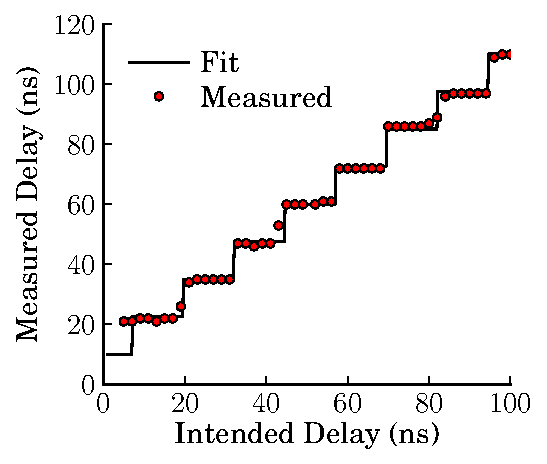
\includegraphics[width=.50\linewidth]{OLTP_eval/Delay.pdf}
  \caption{\textbf{Delay precision.} Delays are implemented by repeatedly reading the TSC register.  Resulting delays form a step function.  Inserted delays are within 6ns of the intended delay.}
  \label{fig::Delay}
\end{figure}

Figure~\ref{fig::Delay} shows the measured delay that results from iterating on an intended delay (both in ns).
Points show the median of ten thousand delay trials (a small number of trials result in excessively large delays and skew the mean).
The delay function resembles a step function---delays may only be inserted in multiples of the loop iteration latency.

To better understand delay behavior I perform a least squares regression of a step function against the measured data of the form:
$$delay(intended) = a \times floor(intended / a + b) + c$$
which results in an $R^2$ of .997 and the following parameter values: $a = 12.5$, $b=.434$, and $c=10.1$.
This indicates that each iteration takes 12.5ns.

As delays can only be introduced in steps I subtract 9.3ns from the intended delay to match to the closest step.
The resulting delay is within 6.25ns of the intended delay.
However, a given delay contains a constant skew (for example, an intended delay of 30ns always results in a 35ns delay).
As NVRAM persist latencies are expected to be in the hundreds of ns or greater, such error will negligibly affect my results.

\textbf{Modeling NVRAM persist bandwidth.}
In addition to NVRAM latency, I model shared NVRAM write bandwidth.
Using RDTSCP as a clock source, I maintain a shared \emph{next\_available} variable, representing the next clock tick in which the NVRAM device is available to be written.
Each NVRAM persist advances \emph{next\_available} to account for the latency of its persist operation.
Reservations take the maximum of \emph{next\_available} and the current RDTSCP and add the reservation duration.
The new value is atomically swapped into \emph{next\_available} via a Compare-And-Swap (CAS).
If the CAS fails (due to a race with a persist operation on another thread), the process repeats until it succeeds.
Upon success, the thread delays until the end of its reservation.
The main limitation of this approach is that it cannot model reservations shorter than the delay required to perform a CAS to a contended shared variable.
The delay incurred by a CAS instruction depends on contention to the address and the scheduling of threads across cores and processors.
I demonstrate that this technique models reservations above 120ns accurately, which is sufficient for my experiments.

Several factors affect the speed of bandwidth reservations (and therefore reservation accuracy) including the number of threads and their placement across sockets and cores.
I test the reservation system's accuracy by constraining thread placement while threads repeatedly reserve time and delay until the end of the reservation.
If all available time is reserved, reservation overhead is negligible and the modeled bandwidth is accurate.
However, when reservation length is sufficiently short reservation overheads will dominate, resulting in unreserved time.

\begin{table*}
  \centering
  \subtable[6 threads]{
    \label{table::Reservation::6}
    \begin{tabular}{l l l}
      \hline
      socket policy & spread cores & pack cores \\
      \hline \hline
      spread & 109 & 122 \\
      pack & 44 & 104 \\
      \hline
      \\
    \end{tabular}
  }
  \subtable[12 threads]{
    \label{table::Reservation::12}
    \begin{tabular}{l l l}
      \hline
      socket policy & spread cores & pack cores \\
      \hline \hline
      spread & 96 & 101 \\
      pack & 51 & 51 \\
      \hline
      \\
    \end{tabular}
  }
  \caption{\textbf{Bandwidth reservation bendmark.} Benchmark repeatedly reserves bandwidth as time and delays until end of the reservation.  Reservations are inaccurate if entire time cannot be reserved (reservation overhead dominates).  Results shown are reservation sizes (in ns) to reserve 99\% time.  We vary thread placement across CPU sockets and cores: packed (fill socket/core before allocating new) or spread (round robin assign to resources).  122ns and greater reservations accurately model constrained bandwidth.}
  \label{table::Reservation}
\end{table*}


Table~\ref{table::Reservation} shows the required reservation length (in ns) to reserve 99\% of time with six and 12 threads.
Additionally, the Table shows different thread placement across sockets and cores.
``Spread" implies assigning threads round-robin to resources, while ``pack" indicates that each resource is filled before assigning any threads to the next.
For example, assigning six threads in a pack sockets--spread cores policy (on a two socket server, each with six cores and two-way SMT) results in all six threads scheduled on the same socket but each thread on its own core (thus SMT is unused).
Such a configuration requires reservations of only 44ns to reserve 99\% of bandwidth-time.

Spreading threads across sockets or packing within cores slows reservations by requiring long-latency communication between sockets or forcing threads to contend with each other while scheduling instructions on cores.
At worst, when threads are spread across sockets and packed within cores a reservation length of 122ns is required to reserve 99\% of time.

A similar trend is true when considering 12 threads.
Packing threads into a socket completely fills all cores and SMT contexts of the socket (the bottom two cells represent the same configuration), needing 51ns reservations for accurate bandwidth modeling.
Spreading threads across sockets while packing cores requires 101ns to reserve 99\% of time.
The required time decreases from six to 12 threads as more threads are available to reserve time and it is less likely that time will go unreserved.

These results suggest that bandwidth reservations will be accurate, regardless of how threads are scheduled across processors and cores, so long as each reservation exceeds 120ns.
My additions to Shore-MT reserve bandwidth for each cache line persisted.
The persist bandwidth analysis study (presented later in Section~\ref{sec:OLTP_eval:Persists:Limitations}) shows that 35ns per cache line (approximately 1.7GB/s persists) represents sufficient bandwidth to negligibly limit performance.
Since at least four cache lines are always reserved together (in \texttt{persist\_page} and \texttt{persist\_wal}) the bandwidth reservation is accurate.

\textbf{NVRAM performance.}
I introduce NVRAM read and write delays separately.
Accurately modeling per-access increases in read latency is challenging, as reads are frequent and the expected latency increases on NVRAM compared to DRAM are small.
It is infeasible to use software instrumentation to model such latency increases at the granularity of individual reads; hardware support, substantial time dilation, or alternative evaluation techniques (e.g., simulation) would be required, all of which compromise accuracy and the ability to run experiments at full scale.
Instead, I use offline analysis with PIN \cite{LukCohn05} to determine (1) the reuse statistics of buffer cache pages, and (2) the average number of cache lines accessed each time a page is latched.
Together, these offline statistics provide an average number of cache line accesses per page latch event in Shore-MT.
I then introduce a delay at each latch based on the measured average number of misses and an assumed per-read latency increase based on the NVRAM technology.

I model NVRAM persist delays by annotating Shore-MT to track buffer cache writes at cache line granularity---64 bytes---using efficient ``dirty" bitmaps.
Depending on the recovery mechanism, I introduce delays corresponding to persist barriers and to model NVRAM write bandwidth contention.
Tracking buffer cache writes introduces less than a 3\% overhead to the highest throughput experiments.

I choose on-line timing modeling via software instrumentation in lieu of architectural simulations to allow experiments to execute at full scale and in real time.
While modeling aspects of NVRAM systems such as cache performance and more precise persist barrier delays require detailed hardware simulation, I believe NVRAM device and memory system design are not sufficiently established to consider this level of detail.
Instead, I investigate more general trends to determine if and when NVRAM read and write performance warrant storage management redesign.

\textbf{Recovery performance.} Figure~\ref{fig::Recovery} displays recovery latency vs transaction throughput for the TPCB workload, varying page flush rate.
Page flush rate is controlled by maintaining a constant number of dirty pages in the buffer cache, always flushing the page with the oldest volatile update.
Experiments run TPCB for one minute (sufficient to reach steady state behavior) and then kill the Shore-MT process.
Before starting recovery I drop the file system cache.
Reported recovery time includes only the recovery portion of the Shore-MT process; I do not include system startup time nor non-recovery Shore-MT startup time.

\textbf{Workloads.}
I use three workloads and transactions in this evaluation: TPCC, TPCB, and TATP.
TPCC models order management for a company providing a product or service \cite{TPCC}.
TPCB contains one transaction class and models a bank executing transactions across branches, tellers, customers, and accounts \cite{TPCB}.
TATP includes seven transactions to model a Home Location Registry used by mobile carriers \cite{TATP}.
Table~\ref{table::Workloads} shows the workload configuration.
%I choose a single updating transaction from each workload and size workloads to fit in a 12GB buffer cache.
I scale workloads to fit in a 12GB buffer cache.
Persist performance experiments use a single write-heavy transaction from each workload while read performance experiments use each workload's full mix.
All experiments report throughput as thousands of Transactions Per Second (kTPS).
Experiments perform ``power runs"---each thread generates and executes transactions continuously without think time---and run an optimal number of threads per configuration (between 10 and 12).

\begin{table}
  \centering
  \begin{tabular}{l l l l}
    \hline
    Workload & Scale factor & Size & Write transaction \\
    \hline \hline
    TPCC & 70 & 9GB & New order \\
    TPCB & 1000 & 11GB & \\
    TATP & 600 & 10GB & Update location \\
    \hline
  \end{tabular}
  \caption{\textbf{Workloads and transactions.}  One transaction class from each of three workloads, sized to approximately 10GB.}
  \label{table::Workloads}
\end{table}

\section{NVRAM Reads}
\label{sec:OLTP_eval:Reads}

I first evaluate database performance with respect to NVRAM reads.
Many candidate NVRAM technologies exhibit greater read latency than DRAM, possibly requiring additional hardware or software caching.
I wish to determine, for a given NVRAM read latency, how much caching is necessary to prevent slowdown, and whether it is feasible to provide this capacity in a hardware-controlled cache (otherwise software caches must be used).

\subsection{NVRAM Caching Performance}
\label{sec:OLTP_eval:Reads:Performance}

\textbf{Traces.}
\begin{table*}
  \centering
  \begin{tabulary}{\textwidth}{L L L L L L L L L}
    \hline
    & \multicolumn{2}{c}{TATP} & \multicolumn{2}{c}{TPCB} & \multicolumn{2}{c}{TPCC} & \multicolumn{2}{c}{Average} \\
    & \% lines & lines/latch & \% lines & lines/latch & \% lines & lines/latch & \% lines & lines/latch \\
    \hline \hline
    Store & 10.57\% & 5.32 & 11.71\% & 6.05 & 15.47\% &  4.25 & 12.58\% & 5.20 \\
    Index & 89.43\% & 11.27 & 82.41\% & 12.19 & 81.18\% & 11.17 & 84.34\% & 11.54 \\
    Other & 0.00\% & 0.00 & 5.89\% & 7.16 & 3.36\% & 3.00 & 3.08\% & 3.39 \\
    Total & & 5.53 & & 8.47 & & 6.14 & & 6.71 \\
    \hline
  \end{tabulary}
  \caption{\textbf{NVRAM access characteristics.} ``\% lines" indicates the percentage breakdown of cache line accesses.  ``lines/latch" reports the average number of cache line accesses per page latch.  Indices represent the majority of accesses.}
  \label{table::AccessCharacteristics}
\end{table*}

The NVRAM read-performance model combines memory access trace analysis with the timing model to measure transaction throughput directly in Shore-MT.
Traces consist of memory accesses to the buffer cache, collected running Shore-MT with PIN for a single transaction thread for two minutes.
I assume concurrent threads exhibit similar access patterns.
In addition, I record all latch events (acquire and release) and latch page information (i.e., table id, store type---index, heap, or other).
I analyze traces at cache line (64 bytes) and page (8KB) granularity.

These traces provide insight into how Shore-MT accesses persistent data, summarized in Table~\ref{table::AccessCharacteristics}.
Index accesses represent the great majority of cache line accesses, averaging 85\% of accesses to NVRAM across workloads.
Any caching efforts should focus primarily on index pages and cache lines.
Note also that indexes access a greater number of cache lines per page access than other page types (average 11.48 vs 4.85 for heap pages and 4.77 for other page types), suggesting that uncached index page accesses have the potential to introduce greater delays.

\textbf{Throughput.}
\begin{figure}
  \centering
  \subfigure[TATP]{\label{fig::ReadPerformance::TATP} 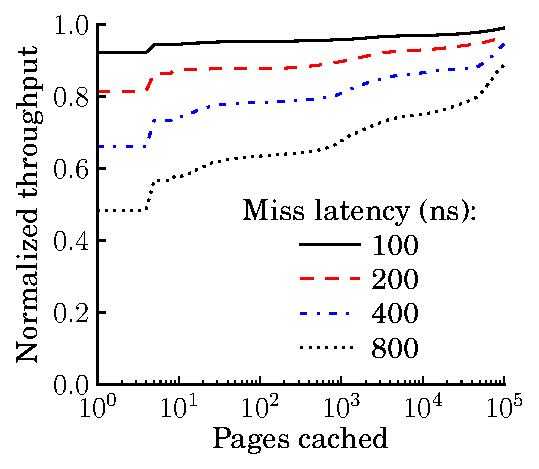
\includegraphics[width=.49\textwidth]{OLTP_eval/ReadPerformance_TATP.pdf}}
  \subfigure[TPCB]{\label{fig::ReadPerformance::TPCB}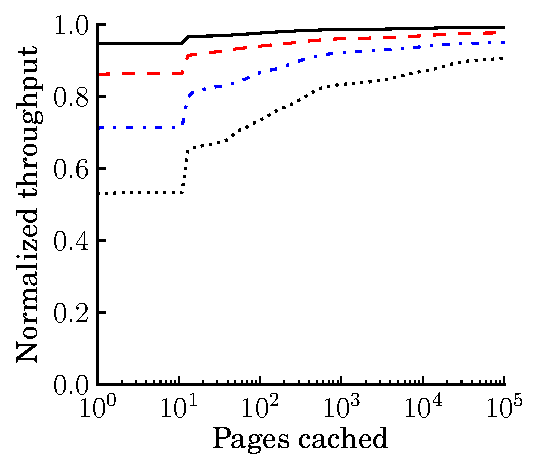
\includegraphics[width=.49\textwidth]{OLTP_eval/ReadPerformance_TPCB.pdf}}
  \subfigure[TPCC]{\label{fig::ReadPerformance::TPCC}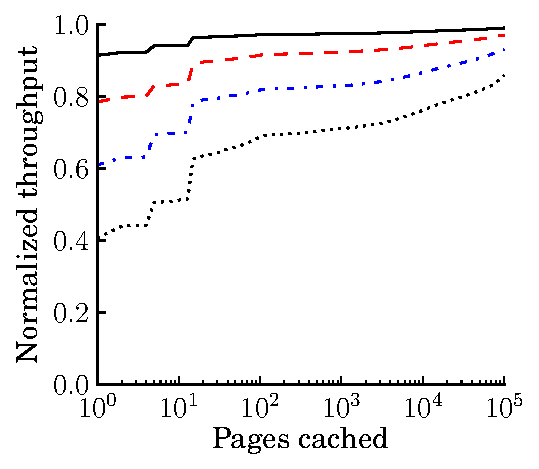
\includegraphics[width=.49\textwidth]{OLTP_eval/ReadPerformance_TPCC.pdf}}
%  \begin{subfigure}{0.32\textwidth}
%    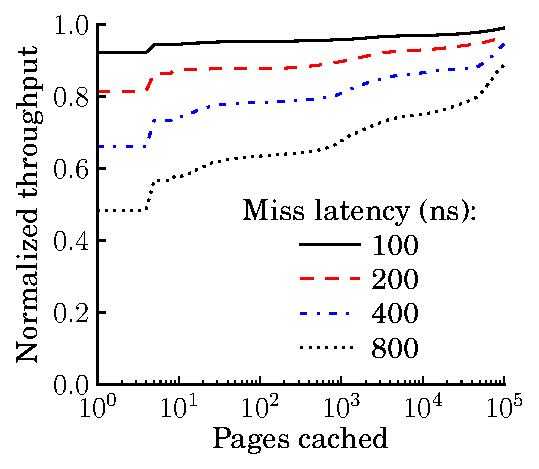
\includegraphics[width=\textwidth]{OLTP_eval/ReadPerformance_TATP.pdf}
%    \caption{TATP}
%    \label{fig::ReadPerformance::TATP}
%  \end{subfigure}
%  \begin{subfigure}{0.32\textwidth}
%    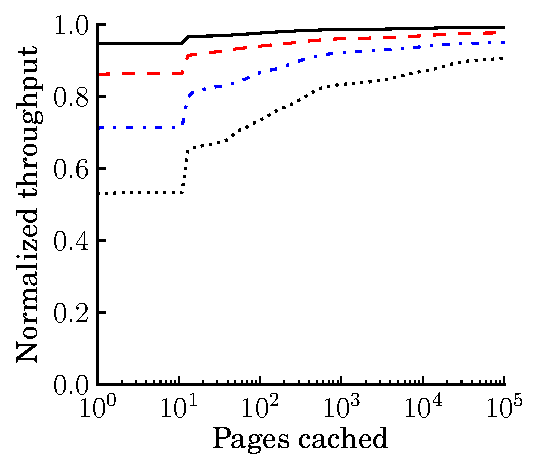
\includegraphics[width=\textwidth]{OLTP_eval/ReadPerformance_TPCB.pdf}
%    \caption{TPCB}
%    \label{fig::ReadPerformance::TPCB}
%  \end{subfigure}
%  \begin{subfigure}{0.32\textwidth}
%    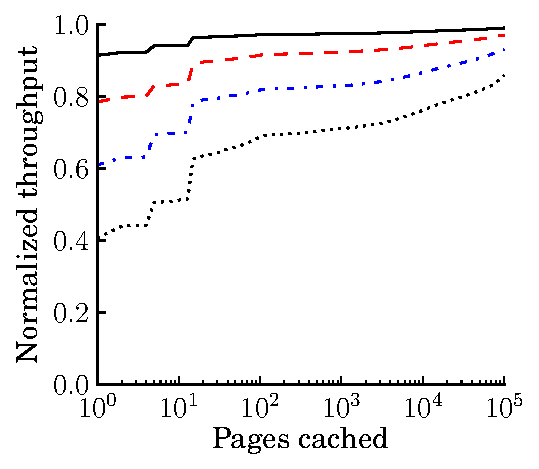
\includegraphics[width=\textwidth]{OLTP_eval/ReadPerformance_TPCC.pdf}
%    \caption{TPCC}
%    \label{fig::ReadPerformance::TPCC}
%  \end{subfigure}
  \caption{\textbf{Throughput vs NVRAM read latency.} 100ns miss latency suffers up to a 10\% slowdown over DRAM.  Higher miss latencies introduce large slowdowns, requiring caching.  Fortunately, even small caches effectively accelerate reads.}
  \label{fig::ReadPerformance}
\end{figure}

I create a timing model in Shore-MT from the previous memory traces.
Given traces, I perform cache analysis at page granularity, treating latches as page accesses and assuming a fully associative cache with a least-recently-used replacement policy (LRU).
Cache analysis produces an average page miss rate to each table.
I conservatively assume that every cache line access within an uncached page introduces an NVRAM stall, neglecting optimizations such as out-of-order execution and simultaneous multi-threading that might hide some NVRAM access stalls. 
The model assumes the test platform incurs a 50ns DRAM fetch latency, and adds additional latency to mimic NVRAM (for example, a 200ns NVRAM access adds 150ns delay per cache line).
I combine average page miss rate and average miss penalty (from lines/latch in table~\ref{table::AccessCharacteristics}) to compute the average delay incurred per latch event.
This delay is inserted at each page latch acquire in Shore-MT, using \InPlace, to produce a corresponding throughput.

Figure~\ref{fig::ReadPerformance} shows throughput achieved for the three workloads while varying the number of pages cached (horizontal axis) and NVRAM miss latency (various lines).
The vertical axis displays throughput normalized to DRAM-miss-latency's throughput (no additional delay inserted).
Without caching, throughput suffers as NVRAM miss latency increases, shown at the extreme left of each graph.
A 100ns miss latency consistently achieves at least 90\% of potential throughput.
However, an 800ns miss latency averages only 50\% of the potential throughput, clearly requiring caching.
TPCB and TPCC see a 10-20\% throughput improvement for a cache size of just 20 pages.
As cache capacity further increases, each workload's throughput improves to varying degrees.
A cache capacity of 100,000 (or 819MB at 8KB pages) allows NVRAMs with 800ns miss latencies to achieve at least 80\% of the potential throughput.
While too large for on-chip caches, such a buffer might be possible as a hardware-managed DRAM cache \cite{QureshiSrinivasan09}.

\subsection{Analysis}
\label{sec:OLTP_eval:Reads:Analysis}
\begin{figure}
  \centering
  \subfigure[TATP]{\label{fig::Caching::TATP} 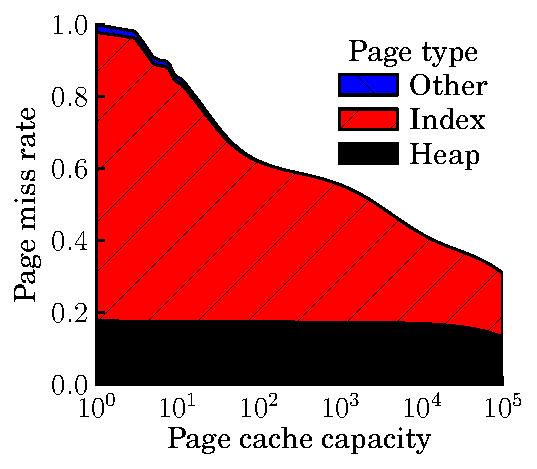
\includegraphics[width=.45\textwidth]{OLTP_eval/Caching_TATP.pdf}}
  \subfigure[TPCB]{\label{fig::Caching::TPCB}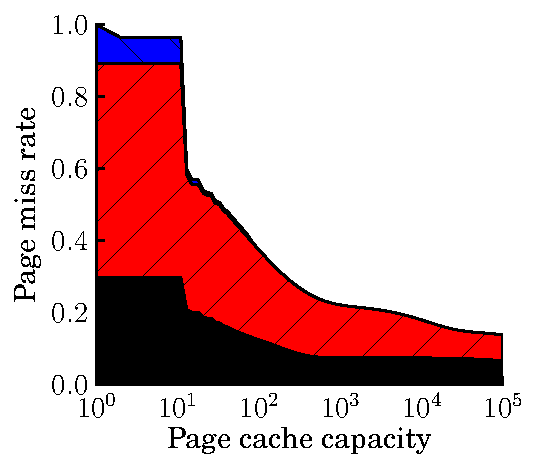
\includegraphics[width=.45\textwidth]{OLTP_eval/Caching_TPCB.pdf}}
  \subfigure[TPCC]{\label{fig::Caching::TPCC}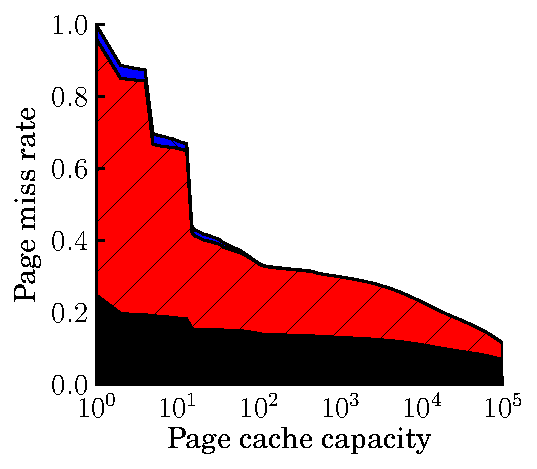
\includegraphics[width=.45\textwidth]{OLTP_eval/Caching_TPCC.pdf}}
  \caption{\textbf{Page caching effectiveness.} High level B+Tree pages and append-heavy store pages cache effectively.  Other pages cache as capacity approaches table size.}
  \label{fig::Caching}
\end{figure}

I have shown that modest cache sizes effectively hide NVRAM read stalls for these workloads, and further analyze caching behavior to reason about OLTP performance more generally.
Figure~\ref{fig::Caching} shows the page miss rate per page type (index, heap, or other) as page cache capacity increases.
Each graph begins at one at the left---all page accesses miss for a single-page cache.
As cache capacity increases, workloads see their miss rates start to decrease between cache capacity of five and 20 pages.
TATP experiences a decrease in misses primarily in index pages, whereas TPCB and TPCC see decreases across all page types.

While cache behavior is specific to each workload, the results represent trends applicable to many databases and workloads, specifically, index accesses and append-heavy tables.
First, all workloads see a decrease in index page misses as soon as B+Tree roots (accessed on every traversal) successfully cache.
The hierarchical nature of B+Tree indexes allows high levels of the tree to cache effectively for even a small cache capacity.
Additionally, TPCB and TPCC contain history tables to which data are primarily appended.
Transactions append to the same page as previous transactions, allowing such tables to cache effectively.
Similarly, extent map pages used for allocating new pages and locating pages to append into are frequently accessed and likely to cache.
The remaining tables' pages are accessed randomly and only cache as capacity approaches the size of each table.
In the case of TPCB and TPCC, each transaction touches a random tuple of successively larger tables (Branch, Teller, and Account for TPCB; Warehouse, District, Customer, etc. for TPCC).
This analysis suggests that various page types, notably index and append-heavy pages, cache effectively, accelerating throughput for high-latency NVRAM misses with small cache capacities.

\textbf{Main-memory databases.}
While I use Shore-MT (a disk-based storage manager) as a research platform, main-memory database optimizations (e.g., \cite{DiaconuFreedman13, BallardBehman11, Oracle09}) also apply to byte-addressable NVRAM.
Main-memory databas\-es assume heap data resides solely in byte-addressable memory, improving throughput relative to traditional disk-back\-ed storage by removing expensive indirection (i.e., using memory pointers instead of buffer translation tables), reducing overheads associated with concurrency control and latches, and optimizing data layout for caches and main-memory, among other optimizations.
While such optimizations will increase transaction throughput, removing non-NVRAM overheads will amplify the importance of read-miss latency (an equal increase in NVRAM read-miss latency will yield a relatively greater drop in performance).
At the same time, data layout optimizations will reduce the number of cache lines and memory rows accessed per action (e.g., per latch), minimizing NVRAM read overheads.
Investigating main-memory database optimizations for NVRAM remains future work.

\begin{table}
  \centering
  \begin{tabular}{l l}
    \hline
    Workload & Bandwidth (GB/s) \\
    \hline \hline
    TATP & 0.977 \\
    TPCB & 1.044 \\
    TPCC & 1.168 \\
    \hline
  \end{tabular}
  \caption{\textbf{Required NVRAM read bandwidth.} Workloads require up to 1.2 GB/s read bandwith.}
  \label{table::ReadBandwidth}
\end{table}

\textbf{Bandwidth.}
Finally, I briefly address NVRAM read bandwidth.
For a worst-case analysis, I assume no caching.
Given the average number of cache line accesses per page latch, the average number of page latches per transaction, and transaction throughput (taken from Section~\ref{sec:OLTP_eval:Persists}), I compute worst-case NVRAM read bandwidth for each workload, shown in Table~\ref{table::ReadBandwidth}.
The considered workloads require at most 1.2 GB/s (TPCC).
Since this is within expected NVRAM bandwidth constraints and caching reduces the required bandwidth further, I conclude that NVRAM read bandwidth for persistent data on OLTP is not a performance concern.

\subsection{Summary}
\label{sec:OLTP_eval:Reads:Summary}
NVRAM presents a new storage technology, requiring new optimizations for database systems.
Increased memory read latencies require new consideration for database caching systems.
I show that persistent data for OLTP can be cached effectively, even with limited cache capacity.
I expect future NVRAM software to leverage hardware caches, omitting software buffer caches.
Next, I turn to write performance for storage management on NVRAM devices.

\section{NVRAM Persist Synchronization}
\label{sec:OLTP_eval:Persists}

Whereas NVRAM reads benefit from caching, persists must always access the storage device.
Of particular insterest is the cost of ordering persists via persist barriers.
Several factors increase persist barrier latency, including ordering persists across distributed/NUMA memory architectures, long latency interconnects (e.g., PCIe-attached storage), and slow NVRAM MLC cell persists.
I consider the effect of persist barrier latency on transaction processing throughput to determine if and when new NVRAM technologies warrant redesigning recovery management.

Refer to Sections~\ref{sec:OLTP_design:Design} and~\ref{sec:OLTP_design:Methodology} for a more thorough description of recovery mechanisms and experimental setup.
All experiments throttle persist bandwidth to 1.5GB/s, which I believe to be conservative (already possible with PCIe-attached Flash).
Ideally, NVRAM will provide low latency access, enabling \InPlace.
However, one would expect \InPlace's performance to suffer at large persist barrier latencies, requiring either \NVDisk or \GroupCommit to regain throughput.

\subsection{Persist Barrier Latency}
\label{sec:OLTP_eval:Persists:Performance}

\begin{figure*}
  \centering
  %\begin{subfigure}{0.32\textwidth}
  %  \includegraphics[width=\textwidth]{figures/pdfs/PersistLatencyThroughput/TATP.pdf}
  %  \caption{TATP}
  %  \label{fig::PersistLatencyThroughput::TATP}
  %\end{subfigure}
  %\begin{subfigure}{0.32\textwidth}
  %  \includegraphics[width=\textwidth]{figures/pdfs/PersistLatencyThroughput/TPCB.pdf}
  %  \caption{TPCB}
  %  \label{fig::PersistLatencyThroughput::TPCB}
  %\end{subfigure}
  %\begin{subfigure}{0.32\textwidth}
  %  \includegraphics[width=\textwidth]{figures/pdfs/PersistLatencyThroughput/TPCC.pdf}
  %  \caption{TPCC}
  %  \label{fig::PersistLatencyThroughput::TPCC}
  %\end{subfigure}
  \subfigure[TATP]{\label{fig::PersistLatencyThroughput::TATP} 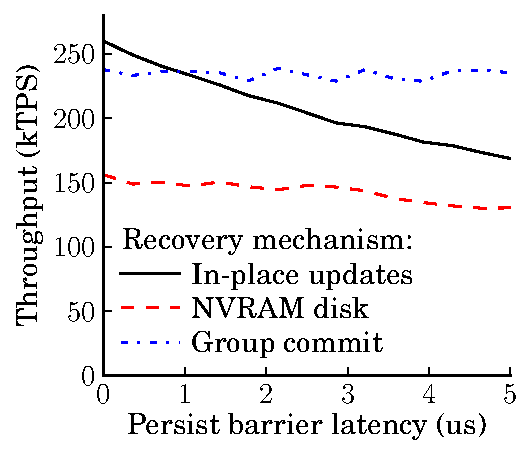
\includegraphics[width=.45\textwidth]{OLTP_eval/PersistLatencyThroughput_TATP.pdf}}
  \subfigure[TPCB]{\label{fig::PersistLatencyThroughput::TPCB}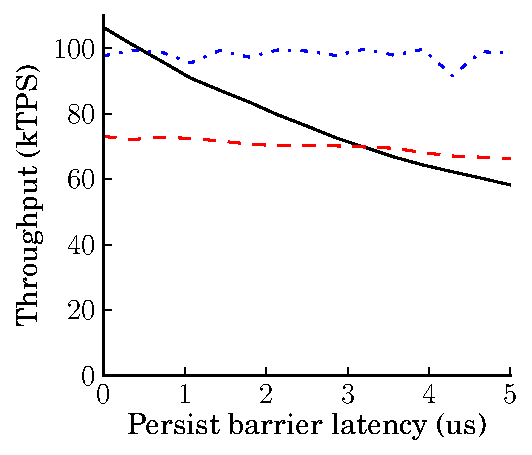
\includegraphics[width=.45\textwidth]{OLTP_eval/PersistLatencyThroughput_TPCB.pdf}}
  \subfigure[TPCC]{\label{fig::PersistLatencyThroughput::TPCC}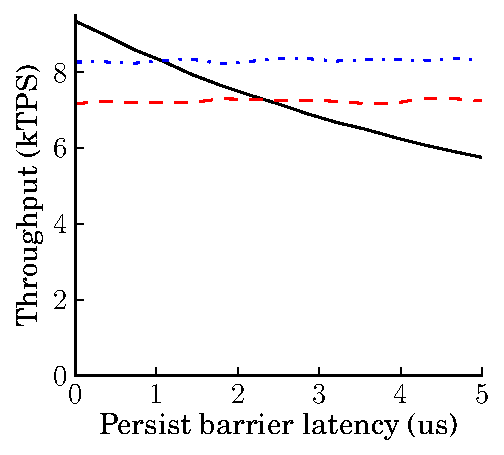
\includegraphics[width=.45\textwidth]{OLTP_eval/PersistLatencyThroughput_TPCC.pdf}}
  \caption{\textbf{Throughput vs persist barrier latency.} \InPlace performs best for zero-cost persist barriers, but throughput suffers as persist barrier latency increases.  \NVDisk and \GroupCommit are both insensitive to increasing persist barrier latency, with \GroupCommit offering higher throughput.}
  \label{fig::PersistLatencyThroughput}
\end{figure*}


Figure~\ref{fig::PersistLatencyThroughput} shows throughput for write-heavy transactions as persist barrier latency increases from 0\textmu s to 5\textmu s, the range believed to encompass realistic latencies for possible implementations of persist barriers and storage architectures.
A persist barrier latency of 0\textmu s (left edge) corresponds to no barrier/DRAM latency.
For such devices (e.g., battery-backed DRAM), \InPlace far out-paces \NVDisk, providing up to a 50\% throughput improvement.
The speedup stems from a combination of removing WAL overheads, removing contention between page flushers and transaction threads, and freeing up (a few) threads from log and page flushers to run additional transactions.
\InPlace also outperforms \GroupCommit, providing an average 10\% throughput improvement across workloads.

As persist barrier latency increases, each recovery mechanism reacts differently.
\InPlace, as expected, loses throughput.
\NVDisk and \GroupCommit, on the other hand, are both insensitive to persist barrier latency; their throughputs see only a small decrease as persist barrier latency increases.
TATP sees the largest throughput decrease for \NVDisk (14\% from 0\textmu s to 5\textmu s).
The decrease stems from \NVDisk's synchronous commits, requiring the log flusher thread to complete flushing before transactions commit.
During this time, transaction threads sit idle.
While both \NVDisk and \GroupCommit retain high throughput, there is a large gap between the two, with \GroupCommit providing up to a 50\% performance improvement over \NVDisk.
This difference, however, is workload dependent, with WAL imposing a greater bottleneck to TATP than to TPCB or TPCC.

Of particular interest are persist barrier latencies where lines intersect---the break-even points for determining the optimal recovery mechanism.
Whereas all workloads prefer \InPlace for a 0\textmu s persist barrier latency, \GroupCommit provides better throughput above 1\textmu s persist barrier latency.
When only considering \InPlace and \NVDisk the decision is less clear.
Over the range of persist barrier latencies TATP always prefers \InPlace to \NVDisk (the break-even latency is well above 5\textmu s).
TPCB and TPCC see the two mechanisms intersect near 3.5\textmu s and 2.5\textmu s, respectively, above which \NVDisk provides higher throughput.
TATP, unlike the other two workloads, only updates a single page per transaction.
Other overheads tend to dominate transaction time, resulting in a relatively shallow \InPlace curve.

\begin{table}
  \centering
  \begin{tabular}{l l l}
    \hline
    Workload & Full mix & Single transaction \\
    \hline \hline
    TATP & 25 & 12 \\
    TPCB & 3.2 & 3.2 \\
    TPCC & 3.6 & 2.4 \\
    \hline
  \end{tabular}
  \caption{\textbf{Break-even persist latency} Persist barrier latency (\textmu s) where \NVDisk and \InPlace achieve equal throughput.  Latencies reported for full transaction mixes and single write-heavy transaction per workload.}
  \label{table::PersistLatencyBreakeven}
\end{table}


The previous results show throughput only for a single transaction from each workload.
Table~\ref{table::PersistLatencyBreakeven} shows break-even persist barrier latency between \NVDisk and \InPlace for these transactions and full transaction mixes.
Full transaction mixes contain read-only transactions, reducing log insert and persist barrier frequency (read-only transactions require no recovery).
\NVDisk sees improved throughput at 0 \textmu s and \InPlace's throughput degrades less quickly as persist barrier latency increases.
As a result, the break-even persist barrier latency between these two designs increases for the full transaction mix relative to a single write-heavy transaction and the opportunity to improve throughput by optimizing recovery management diminishes---improved recovery management does not affect read-only transactions and actions.

These results suggest different conclusions across storage architectures.
NVRAM connected via the main memory bus will provide low latency persist barriers (less than 1\textmu s) and prefer \InPlace.
Other storage architectures, such as distributed storage, require greater delays to synchronize persists.
For such devices, \GroupCommit offers an alternative to \NVDisk that removes software overheads inherent in WAL while providing recovery.
However, \GroupCommit increases transaction latency.

\subsection{Transaction Latency}
\label{sec:OLTP_eval:Persists:XctLatency}

\begin{figure*}
  \centering
  %\begin{subfigure}{0.32\textwidth}
  %  \includegraphics[width=\textwidth]{figures/pdfs/XctLatency/TATP.pdf}
  %  \caption{TATP}
  %  \label{fig::XctLatency::TATP}
  %\end{subfigure}
  %\begin{subfigure}{0.32\textwidth}
  %  \includegraphics[width=\textwidth]{figures/pdfs/XctLatency/TPCB.pdf}
  %  \caption{TPCB}
  %  \label{fig::XctLatency::TPCB}
  %\end{subfigure}
  %\begin{subfigure}{0.32\textwidth}
  %  \includegraphics[width=\textwidth]{figures/pdfs/XctLatency/TPCC.pdf}
  %  \caption{TPCC}
  %  \label{fig::XctLatency::TPCC}
  %\end{subfigure}
  \subfigure[TATP -- Update Location]{\label{fig::XctLatency::TATP} 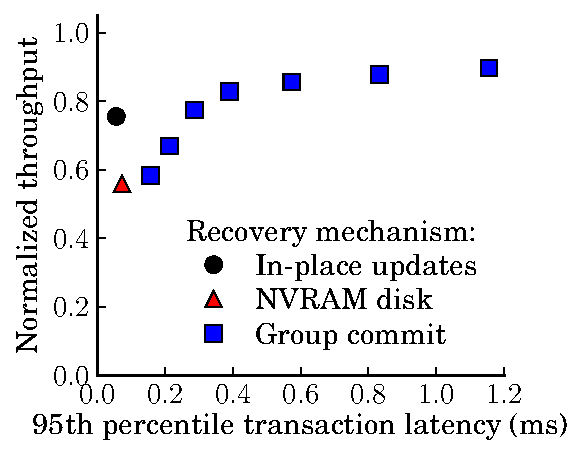
\includegraphics[width=.45\textwidth]{OLTP_eval/XctLatency_TATP.pdf}}
  \subfigure[TPCB]{\label{fig::XctLatency::TPCB}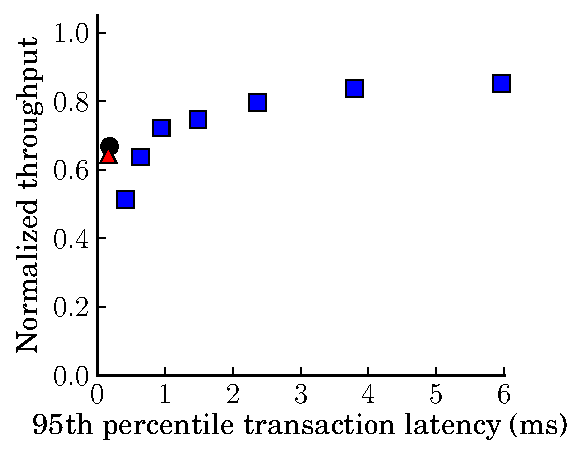
\includegraphics[width=.45\textwidth]{OLTP_eval/XctLatency_TPCB.pdf}}
  \subfigure[TPCC -- New Order]{\label{fig::XctLatency::TPCC}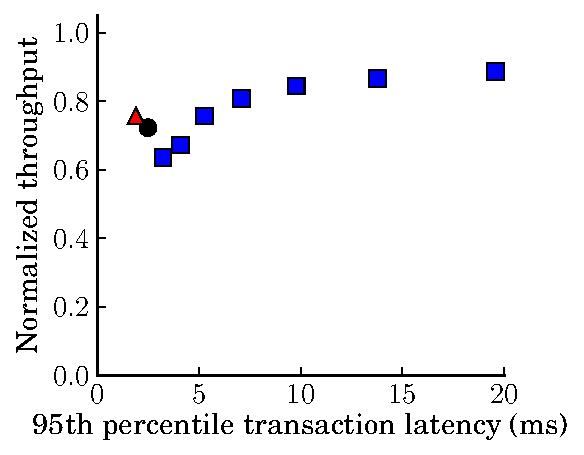
\includegraphics[width=.45\textwidth]{OLTP_eval/XctLatency_TPCC.pdf}}
  \caption{\textbf{95th percentile transaction latency.} All graphs are normalized to 0\textmu s persist barrier latency \InPlace throughput.  Experiments use 3\textmu s persist barrier latency.  \GroupCommit avoids high latency persist barriers by defering transaction commit, committing entire batches atomically.}
  \label{fig::XctLatency}
\end{figure*}


\GroupCommit improves transaction throughput by placing transactions into batches and committing all transactions in a batch atomically.
Doing so minimizes and limits the number of persist barriers.
However, deferring transaction commit increases transaction latency, especially for the earliest transactions in each batch.
To achieve reasonable throughput, batches must be significantly longer than average transaction latency (such that batch execution time dominates batch quiesce and persist time).
The batch period acts as a knob for database administrators to trade off transaction latency and throughput.
I use this knob to measure the relationship between throughput and high-percentile transaction latency.

Figure~\ref{fig::XctLatency} shows throughput, normalized to \InPlace at 0\textmu s persist barrier latency.
The results consider a 3\textmu s persist barrier latency, where \GroupCommit provides a throughput improvement over other recovery mechanisms.
The different \GroupCommit points represent different batch periods, and I report the measured 95th percentile transaction latency for all recovery mechanisms.
I measure transaction latency from the time a transaction begins to the time its batch ends (Shore-MT does not model any pre-transaction queuing time).

The results illustrate that \GroupCommit is capable of providing equivalent throughput to the other recovery mechanisms with reasonable latency increases (no more than 5\texttimes).
Further, high-percentile transaction latencies fall well below the latency expectations of modern applications.
TPCC, the highest latency workload, approaches optimal throughput with a 95th percentile transaction latency of 15ms---similar to latencies incurred by disk-backed databases.
For latency sensitive workloads, the batch period can be selected to precisely control latency, and \InPlace and \NVDisk remain alternatives.

\subsection{NVRAM Persist Limitations}
\label{sec:OLTP_eval:Persists:Limitations}

In addition to persist delays NVRAM may suffer limitations due to persist bandwidth and write endurance.
I quantify these limitations and determine how database design affects each.

\textbf{Persist bandwidth.}
Different NVRAM storage architectures impose a variety of limitations on persist bandwidth (e.g., memory bus-attached NVRAM will allow greater throughput than PCIe-attached NVRAM).
Different software designs place varying requirements on bandwidth.

\begin{figure}
  \centering
  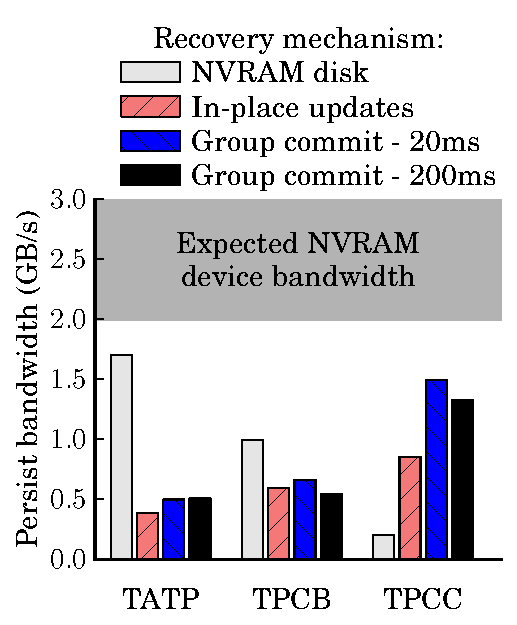
\includegraphics[width=.9\linewidth]{OLTP_eval/Bandwidth.pdf}
  \caption{\textbf{Required NVRAM bandwidth.} Persist/write bandwidth required to achieve 95\% performance relative to no bandwidth constraint.  Bandwidth requirements are far below expected device bandwidth.}
  \label{fig::Bandwidth}
\end{figure}

Figure~\ref{fig::Bandwidth} shows the bandwidth required for each workload and recovery mechanism to achieve 95\% throughput compared to same configuration with no bandwidth constraint.
Each recovery mechanism sees different bandwidth requirements, and required bandwidth varies across workloads.

The \NVDisk configuration flushes pages aggressively (attempts to flush continuously) and consumes all available bandwidth.
Since bandwidth is restricted recovery latency may increase (not reflected in the results).
Page flushing contends with log flushing for bandwidth, but so long as log flushes are minimally delayed throughput will not be affected.
TATP, which contains short transactions, requires the most bandwidth (1.7GB/s) to reduce transaction commit delays.
I believe that asynchronous commit (allowing a new transaction to begin processing on the hardware thread while the previous transaction waits to commit) would lower the bandwidth requirement.
TPCC, on the other hand, has long transactions and transaction commit is less of a concern.

\InPlace requires the least bandwidth of the recovery mechanisms.
TATP's Update Location transaction needs only 0.4GB/s since each transaction contains a single small update.
TPCC's New Order transaction modifies much more data, requiring 0.8GB/s persist bandwidth to achieve 95\% throughput.

Finally, \GroupCommit sees varying requirements on persist bandwidth.
All persists occur at batch boundaries, resulting in persist bursts.
I consider two batch periods---20ms and 200ms.
TATP and TPCC require relatively small bandwidths while TPCC requires over 1.5GB/s persist bandwidth to achieve 95\% throughput.
The bursty nature of \GroupCommit and large modifications by TPCC's New Order transaction result in persist bandwidth quickly creating a bottleneck.
Longer batches help slightly by allowing updates to coalesce within the batch, reducing the total number of bytes persisted.
The bandwidth requirements would be reduced by introducing mechanisms to enable early persists (persist data before the batch ends), removing persist bursts.

While persist bandwidth requirements vary, the strictest configuration (\NVDisk for TATP) requires only 1.7GB/s.
Such bandwidth is currently possible with existing PCIe Flash memory SSDs, and I believe is attainable for all candidate NVRAM technologies.
I expect that persist bandwidth will not be a concern for OLTP systems using NVRAM.

\textbf{Device lifetime.}
NVRAM technologies, much like Flash memory currently, will have limited write endurance; each cell may only be reliably written a finite number of times.
Device lifetime is generally determined by the most frequently written addresses.
Previous work proposes hardware techniques to evenly distribute writes amongst cells by constantly changing the mapping between between memory addresses and the underlying memory cell \cite{QureshiKaridis09}.
These techniques prolong device lifetime by ensuring that frequently written addresses do not wear out individual cells.
While the recovery mechanisms presented here each produce varying persist rates with different abilities to naturally distribute persists across addresses, it is unclear if software mechanisms are sufficient to prolong device lifetime.

\begin{figure*}
  \centering
  \subfigure[No wear leveling]{\label{fig::WearLeveling::None} 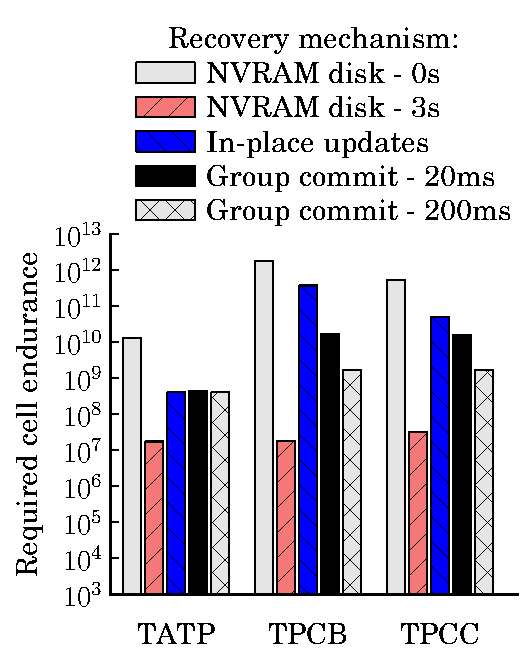
\includegraphics[width=.49\textwidth]{OLTP_eval/WearLeveling_None.pdf}}
  \subfigure[Perfect wear leveling]{\label{fig::WearLeveling::Perfect}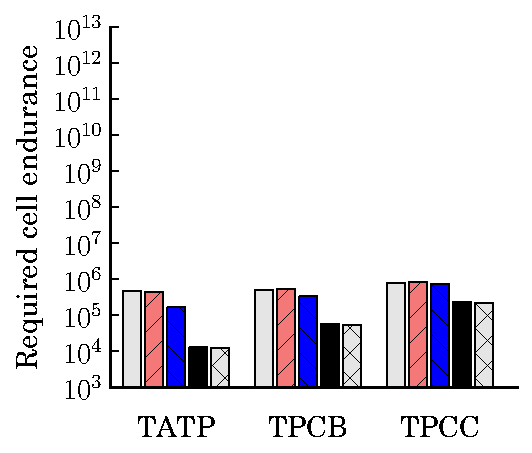
\includegraphics[width=.49\textwidth]{OLTP_eval/WearLeveling_Perfect.pdf}}
  \caption{\textbf{NVRAM cell endurance for 10-year lifetime.}  Without hardware wear leveling the most-written cell limits device lifetime.  \NVDisk requires conservative page flushing (3s recovery latency vs 0s, instantaneous, recovery) and \GroupCommit requires longer batch periods (200ms vs 20ms) to improve device lifetime.  We expect hardware wear leveling to always be required with \InPlace.  With perfect wear leveling (all writes occur evenly throughout cells in the device) and a 32GB storage device all workloads and configurations achieve a 10-year device lifetime for cell endurance of $10^6$ writes and greater.}
  \label{fig::WearLeveling}
\end{figure*}

Figure~\ref{fig::WearLeveling} shows the required cell endurance (number of persists) to achieve a 10-year device lifetime assuming the database runs at maximum throughput continuously.
All recovery mechanisms assume \InPlace's throughput for a more fair comparison.
Persists are tracked at byte granularity.
I consider two scenarios: no wear leveling---lifetime is limited by the most frequently written address---and perfect wear leveling---all persists are evenly distributed across all physical addresses (provided in hardware).
I consider \NVDisk with both instantaneous recovery and 3s recovery latency, \InPlace, and \GroupCommit with 20ms and 200ms batch latencies.
Logs are implemented as circular buffers.
Thus, logs do not contribute to the most written byte and have no bearing on device lifetime when hardware wear leveling is unavailable.
Perfect wear leveling assumes a 32GB device.

Without hardware wear leveling \NVDisk with instantaneous recovery (aggressive page flushing) and \InPlace require the greatest cell endurance.
Both mechanisms persist each update directly to the NVRAM store.
\NVDisk must additionally persist LSNs, which constitute the most frequently persisted addresses, while LSNs are no longer used with \InPlace and \GroupCommit.
Both of these configurations require greater cell endurance far greater than $10^8$ writes, the endurance expected of phase change memory \cite{BurrKurdi08}.

\NVDisk with 3s recovery latency requires much lower cell endurance for a 10 year lifetime.
Writes to heap pages coalesce and only occasionally persist to NVRAM.
\NVDisk effectively increases device lifetime by reducing the total number of persists and limiting the rate that any single page may write back.
However, doing so requires an increase in recovery latency.
\NVDisk may possibly provide acceptable software wear leveling so long as recovery latency is reasonable.

Finally, \GroupCommit provides wear leveling by only allowing a single persist to each address per batch (all other persists coalesce).
However, neither 20ms nor 200ms batches is capable of coalescing enough writes to guarantee a 10 year device lifetime.
\GroupCommit would require far too large a batch period, increasing transaction latency, to reliably wear-level NVRAM.

When hardware distributes persists evenly across NVRAM cells all recovery mechanisms achieve a 10 year lifetime assuming $10^8$ writes per cell.
In this case lifetime is determined by the total number of persists rather than the most-persisted address.
Due to the inability of software to reliably and sufficiently extend device lifetime, and the effectiveness of hardware wear leveling, I expect future NVRAM SSDs to include hardware wear leveling.

\subsection{Summary}
\label{sec:OLTP_eval:Persists:Summary}
Persist barriers used to enforce persist order pose a new performance obstacle to providing recoverable storage management with NVRAM.
I show that, for memory bus-attached NVRAM devices, ensuring recovery using \InPlace is a viable strategy that provides high throughput and removes the overheads of WAL.
For interconnects and NVRAM technologies that incur larger persist barrier delays, \GroupCommit offers an alternative that yields high throughput and reasonable transaction latency.
\GroupCommit's batch period allows precise control over transaction latency for latency-critical applications.
Finally, I demonstrate that persist bandwidth is not a concern, and that while \NVDisk may provide an effective mechanism to cope with limited write endurance I expect future devices to include hardware wear leveling.

%\section{Proposed Work}
%\label{sec:OLTP_eval:Proposed}
%
%I propose to include two additional studies.
%These studies were originally conducted for an earlier journal submission; the experimental system has changed substantially since then.
%
%\textbf{Persist bandwidth.}
%\begin{figure}
  \centering
  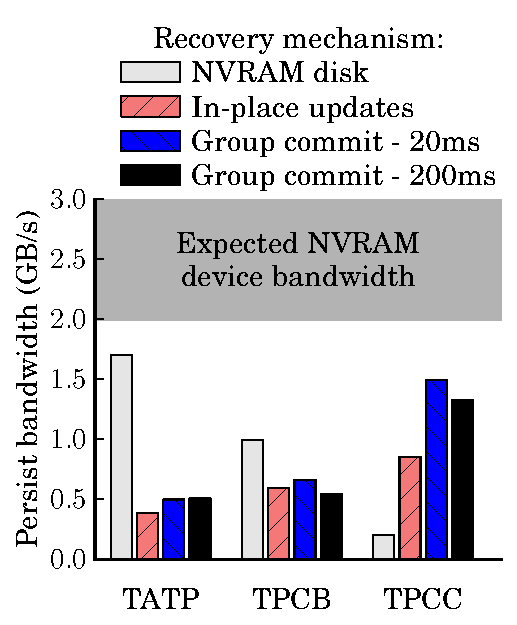
\includegraphics[width=.9\linewidth]{OLTP_eval/Bandwidth.pdf}
  \caption{\textbf{Required NVRAM bandwidth.} Persist/write bandwidth required to achieve 95\% performance relative to no bandwidth constraint.  Bandwidth requirements are far below expected device bandwidth.}
  \label{fig::Bandwidth}
\end{figure}

%Different NVRAM storage architectures impose a variety of limitations on persist bandwidth (e.g., memory bus-attached NVRAM will allow greater throughput than PCIe-attached NVRAM).
%I intend to study the persist bandwidth requirements for each recovery mechanism.
%
%Recovery mechanisms display interesting behaviors with respect to bandwidth.
%\NVDisk persists inefficiently with respect to the total number of bytes updated; even a small page update requires large log entries.
%However, the log persist makes effective use of cache lines (the granularity that data must transfer to the memory device).
%Further, when increased recovery latency is allowable, bandwidth usage may be decreased by deferring page flushing, allowing writes to coalesce in pages.
%The result is that \NVDisk makes reasonable use of bandwidth, and bandwidth constraints are unlikely to limit throughput.
%
%\InPlace displays similar bandwidth usage to \NVDisk.
%All page updates must persist to NVRAM, and these updates tend to use cache lines ineffectively (only a small portion of each cache line changes).
%Also similarly to \NVDisk, \InPlace must maintain ARIES logs (although per-transaction and undo-only), requiring large persists.
%
%\GroupCommit, while persisting the least amount of data, is the most sensitive to persist bandwidth constraints.
%The total quantity of data is reduced by using physical logs -- logs copy data with little associated metadata.
%Additionally, updates in each batch coalesce.
%Only the first write to a given address produces undo, and only the final write to that address persists in-place.
%Other versions of data during the batch do not persist.
%The downside of \GroupCommit is that persists occur in bursts between batches.
%No data persists while the batch executes.
%Between batches however, all logs and heap data persists, placing huge requirements on bandwidth.
%I intend to include a quantitative study of this behavior.
%
%\textbf{Device lifetime.}
%\begin{figure*}
  \centering
  \subfigure[No wear leveling]{\label{fig::WearLeveling::None} 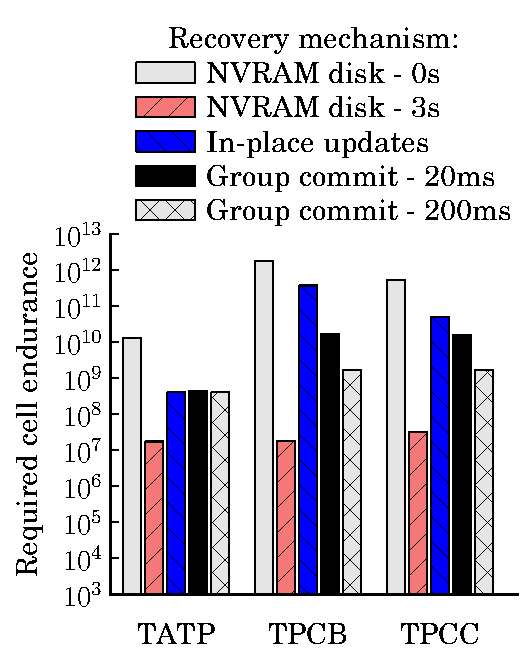
\includegraphics[width=.49\textwidth]{OLTP_eval/WearLeveling_None.pdf}}
  \subfigure[Perfect wear leveling]{\label{fig::WearLeveling::Perfect}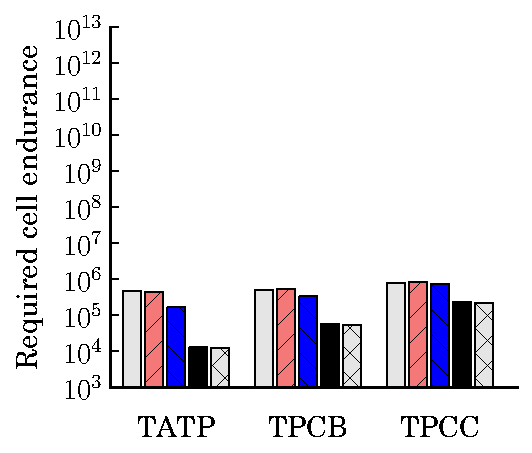
\includegraphics[width=.49\textwidth]{OLTP_eval/WearLeveling_Perfect.pdf}}
  \caption{\textbf{NVRAM cell endurance for 10-year lifetime.}  Without hardware wear leveling the most-written cell limits device lifetime.  \NVDisk requires conservative page flushing (3s recovery latency vs 0s, instantaneous, recovery) and \GroupCommit requires longer batch periods (200ms vs 20ms) to improve device lifetime.  We expect hardware wear leveling to always be required with \InPlace.  With perfect wear leveling (all writes occur evenly throughout cells in the device) and a 32GB storage device all workloads and configurations achieve a 10-year device lifetime for cell endurance of $10^6$ writes and greater.}
  \label{fig::WearLeveling}
\end{figure*}

%NVRAM technologies, much like Flash memory currently, will have limited write endurance; each cell may only be reliably written to a finite number of times.
%Device lifetime is generally determined by the most frequently written addresses.
%Previous work proposes hardware techniques to evenly distribute writes amongst cells by constantly changing the mapping between between memory addresses and the underlying memory cell \cite{QureshiKaridis09}.
%These techniques prolong device lifetime by ensuring that frequently written addresses do not wear out individual cells.
%While the recovery mechanisms presented here each produce varying persist rates with different abilities to naturally distribute persists across addresses, it is unclear if software mechanisms are sufficient to prolong device lifetime.
%I intend to study expected device lifetime for each recovery mechanism, both assuming that persists to an address always persist to the same cell, and assuming hardware that evenly distributes persists across cells.
%
%When wear-leveling hardware is unavailable \NVDisk manages to prolong lifetime the best of the three recovery mechanisms.
%Centralized logs evenly persist to the entire log address space.
%Writes to individual pages may be bounded by limiting the page flush rate, although at the cost of recovery latency.
%\InPlace provides the shortest device lifetime.
%Updates to hot pages and addresses persist each distinct value, quickly wearing out hot cells.
%\GroupCommit limits writes to hot address, but is insufficient to provide lifetime guarantees for expected phase-change write endurance.
%Persists coalesce within each batch, bounding persists to a single write per cell per batch.
%However, batches are sufficiently short that hot addresses still experience a high write-rate, wearing out quickly.
%
%The story changes when hardware spreads persists across NVRAM cells.
%With wear-leveling the primary concern is the total number of persists; all cells experience the same number of persists.
%While \GroupCommit outperforms \NVDisk and \InPlace in this regard, none of the recovery mechanisms pose a device lifetime concern.
%Simply put, an insufficient amount of data persists to worry about device lifetime in the presence of hardware wear-leveling.
%I will include a quantitative evaluation of device lifetime by measuring the rate that persists occur to individual addresses.

\section{Conclusion}
\label{sec:OLTP_eval:Conclusion}
New NVRAM technologies offer an alternative to disk that provides high performance while maintaining durable transaction semantics, yet existing database software is not optimized for such storage devices.
In this chapter, I evaluated recovery management to optimize for NVRAM read and persist characteristics.
I found that even small caches effectively reduce NVRAM read stalls.
I also considered database performance in the presence of persist barrier delays.
Treating NVRAM as a drop-in replacement for disk, \NVDisk retains centralized logging overheads.
\InPlace reduces these overheads, but for large persist barrier latencies suffers from excessive synchronization stalls.
I proposed a new recovery mechanism, \GroupCommit, to minimize these stalls while still removing centralized logging.
While \GroupCommit increases high-percentile transaction latency, latency is controllable and within modern application constraints.

This work assumed that persist barriers are expensive, stalling instruction and thread execution at each barrier.
However, it is possible for systems to implement high performance barriers that overlap instruction execution with persists while still enforcing proper persist order.
Additionally, persist barriers must interact with existing memory execution and the memory consistency model to enforce an order between persists from different threads.
The remainder of this dissertation investigates programming interfaces that to enforce persist order while still maximizing persist concurrency.


\startappendices
 \appendix{Two-Dimensional Crank-Nicolson Scheme for a Uniform Spherical Grid}
 \label{app:CN Scheme}
 This is an example appendix.
For the diffusion process, The equation was solved using a two-dimensional implicit Crank-Nicolson scheme, which is unconditionally stable and second-order accurate in both time and space \citep{crank47}. In the conventional notation, the two-dimensional numerical scheme using central differencing can be written for a uniform Cartesian grid as 
\begin{eqnarray}
\nonumber\left(1+2\mu\right)u^{t+1}_{i,j}-\frac{\mu}{2}\left(u^{t+1}_{i+1,j}+u^{t+1}_{i-1,j}+u^{t+1}_{i,j+1}+u^{t+1}_{i,j-1}\right)\\
=\left(1-2\mu\right)u^{t}_{i,j}+\frac{\mu}{2}\left(u^{t}_{i+1,j}+u^{t}_{i-1,j}+u^{t}_{i,j+1}+u^{t}_{i,j-1}\right),
\end{eqnarray}

\noindent where $u^{t}_{i,j}$ is the value of the parameter undergoing the diffusion ($B_{r}$ in this case) at position $(i, j)$ at time \textit{t}. The von Neumann number on a uniform grid is $\mu=\xi{\Delta}t/\left({\Delta}x\right)^{2}$, where the size of the grid square is $\Delta x$ on each side, and the diffusion coefficient $\xi$ describes the speed at which the mathematical diffusion takes place. When deriving the two-dimensional Crank-Nicolson scheme in spherical coordinates, the von Neumann number is written as $\mu=\xi{\Delta}t/\left(r\Delta\theta\right)^{2}$, where $\Delta\theta=\Delta\phi$, and the cosine is replaced by the central difference of the sine to remain consistent with the discrete nature of the other terms. Care must be taken at the poles, where the central differencing is replaced by forward or backward differencing. To keep second-order accuracy with forward or backward differencing, the series must be carried out to higher-order terms in the derivation. The two-dimensional numerical scheme using central differencing can be written for a uniform spherical grid as
\begin{multline}
\left(1+\mu+\frac{\mu}{\sin^{2}\theta_{i,j}}\right)u^{t+1}_{i,j}-\frac{\mu}{2}\left[1+\frac{\left(\sin\theta_{i+1,j}-\sin\theta_{i-1,j}\right)}{4\sin\theta_{i,j}}\right]u^{t+1}_{i+1,j}\\
 -\frac{\mu}{2}\left[1-\frac{\left(\sin\theta_{i+1,j}-\sin\theta_{i-1,j}\right)}{4\sin\theta_{i,j}}\right]u^{t+1}_{i-1,j}-\frac{\mu}{2}\frac{1}{\sin^{2}\theta_{i,j}}u^{t+1}_{i,j+1}-\frac{\mu}{2}\frac{1}{\sin^{2}\theta_{i,j}}u^{t+1}_{i,j-1}\\
 =\left(1-\mu-\frac{\mu}{\sin^{2}\theta_{i,j}}\right)u^{t+1}_{i,j}+\frac{\mu}{2}\left[1+\frac{\left(\sin\theta_{i+1,j}-\sin\theta_{i-1,j}\right)}{4\sin\theta_{i,j}}\right]u^{t+1}_{i+1,j}\\
 +\frac{\mu}{2}\left[1-\frac{\left(\sin\theta_{i+1,j}-\sin\theta_{i-1,j}\right)}{4\sin\theta_{i,j}}\right]u^{t+1}_{i-1,j}+\frac{\mu}{2}\frac{1}{\sin^{2}\theta_{i,j}}u^{t+1}_{i,j+1}+\frac{\mu}{2}\frac{1}{\sin^{2}\theta_{i,j}}u^{t+1}_{i,j-1}.
 \label{CN Spherical}
\end{multline}

%Although it is unconditionally stable, a marching scheme such as this will depend on the value of $\mu$ for its accuracy. A lower choice of $\mu$ will lead to a more accurate solution at the expense of computational resources (i.e., a smaller time step ${\Delta}t$), while a higher value of $\mu$ will arrive at a solution more rapidly but with less accuracy (a larger time step). In this model, the value of the coefficient $\xi$ describes the speed of the mathematical relaxation and, since it does not describe a physical process, can be chosen arbitrarily. Thus the only restriction for this scheme will lie in keeping $\mu$ small for accuracy and assigning either $\xi$ or ${\Delta}t$. It can be seen that when $\mu$ is held constant, any choice for either $\xi$ or ${\Delta}t$ will lead to the same solution. A value of $\mu=1/4$ was chosen, with an arbitrary time step of ${\Delta}t=0.1$ s, and studied several different grid resolutions, with a grid size of 2.5$^\circ$ x 2.5$^\circ$ (72 x 144 grid spaces) on a uniform spherical grid used for the comparisons in this paper. The relaxation was allowed to continue on a sphere of $r=R_{\sun}$ until the difference in magnetic field magnitude between any cell and its neighbor was of order $10^{-1}{\mu}T$.

 
\startbibliography
 \begin{singlespace} % Bibliography must be single spaced
  \bibliography{References}   % Use the BibTeX file ``References.bib''.
 \end{singlespace}

% An external Abstract that can be printed at the end of the document, 
% for separate submission to Rackham. Comment it out when not needed. - jg
%\startextabstractpage
%{The Title of Your Dissertation}{Your Name}{Chair: Albert Einstein}
%Emerging storage technologies offer an alternative to disk that is durable and allows faster data access.
Flash memory, made popular by mobile devices, provides block access with low latency random reads.
New nonvolatile memories (NVRAM) are expected in upcoming years, presenting DRAM-like performance alongside persistent storage.
Wheres both technologies accelerate data accesses due to increased raw speed, used merely as disk replacements they may fail to achieve their full potentials.
Flash's asymmetric read/write access (i.e., reads execute faster than writes) opens new opportunities to optimize Flash-specific access.
Similarly, NVRAM's low latency persistent accesses allow new designs for high performance failure-resistant applications.

This thesis addresses software and hardware system design for such storage technologies.
First, I investigate analytics query optimization for Flash, expecting Flash's fast random access to require new query planning.
While intuition suggests scan and join selection should shift between disk and Flash, I find that query plans chosen assuming disk are already near-optimal for Flash.
Second, I examine new opportunities for durable, recoverable transaction processing with NVRAM.
Existing disk-based recovery mechanisms impose large software overheads, yet updating data in-place requires frequent device synchronization that limits throughput.
I introduce a new design, \GroupCommit, to amortize synchronization delays over many transactions, increasing throughput at some cost to transaction latency.
Finally, I propose a new framework for persistent programming and memory systems to enable high performance recoverable data structures with NVRAM, extending memory consistency with persistent semantics to introduce \emph{memory persistency}.

%\label{ExtAbstract}

\end{document}
